%%%%%%%%%%%%%%%%%%%%%%%%%%%%%%%%%%%%%%%%%%%%%%%%%%%%%%%%%%%%%%%%%%%%%%%%%%%%
% AGUJournalTemplate.tex: this template file is for articles formatted with LaTeX
%
% This file includes commands and instructions
% given in the order necessary to produce a final output that will
% satisfy AGU requirements, including customized APA reference formatting.
%
% You may copy this file and give it your
% article name, and enter your text.
%
%
% Step 1: Set the \documentclass
%
%

%% To submit your paper:
\documentclass{article}
\usepackage{url} %this package should fix any errors with URLs in refs.
\usepackage{lineno}
\usepackage[inline]{trackchanges} %for better track changes. finalnew option will compile document with changes incorporated.
\usepackage{soul}
\usepackage{hyperref}
\usepackage{natbib}
\usepackage{amsmath}
\usepackage{amssymb}
\usepackage{graphicx}
\usepackage[margin=1in]{geometry}
\newcommand{\bs}{\boldsymbol{s}}
\newcommand{\bg}{\boldsymbol{g}}
\newcommand{\bh}{\boldsymbol{h}}

% \linenumbers

\newcommand{\apbc}{\textit{a priori} bias correction }

%%%%%%%
% As of 2018 we recommend use of the TrackChanges package to mark revisions.
% The trackchanges package adds five new LaTeX commands:
%
%  \note[editor]{The note}
%  \annote[editor]{Text to annotate}{The note}
%  \add[editor]{Text to add}
%  \remove[editor]{Text to remove}
%  \change[editor]{Text to remove}{Text to add}
%
% complete documentation is here: http://trackchanges.sourceforge.net/
%%%%%%%

% \draftfalse

%% Enter journal name below.
%% Choose from this list of Journals:
%
% JGR: Atmospheres
% JGR: Biogeosciences
% JGR: Earth Surface
% JGR: Oceans
% JGR: Planets
% JGR: Solid Earth
% JGR: Space Physics
% Global Biogeochemical Cycles
% Geophysical Research Letters
% Paleoceanography and Paleoclimatology
% Radio Science
% Reviews of Geophysics
% Tectonics
% Space Weather
% Water Resources Research
% Geochemistry, Geophysics, Geosystems
% Journal of Advances in Modeling Earth Systems (JAMES)
% Earth's Future
% Earth and Space Science
% Geohealth
%
% ie, \journalname{Water Resources Research}

% \journalname{Geophysical Research Letters}
\def\authors#1{{\centering \normalsize\bf #1\vskip12pt}}
\def\affil#1{$^{#1}$\ignorespaces}
\def\affiliation#1#2{\vskip-.5\parskip\relax{\centering{\footnotesize
$^{#1}$#2\relax}\vskip-\parskip}}


\begin{document}
\renewcommand{\thefigure}{S\arabic{figure}}
\renewcommand{\thetable}{S\arabic{table}}
\linenumbers

% Track changes
\newcommand{\newTxt}{\textcolor{red}}

% Hide previous edits
% \newcommand{\sti}[1]{\unskip}
% \newcommand{\newTxt}{\textcolor{black}}


%% ------------------------------------------------------------------------ %%
%  Title
%
% (A title should be specific, informative, and brief. Use
% abbreviations only if they are defined in the abstract. Titles that
% start with general keywords then specific terms are optimized in
% searches)
%
%% ------------------------------------------------------------------------ %%

% Example: \title{This is a test title}

\title{Supporting Information for:\\Surface temperature extremes produced by huge machine learning hindcasts of summer 2023}
\date{}
\maketitle

\authors{Mark Risser\affil{1,*}, Ankur Mahesh\affil{1,2,*}, Joshua North\affil{1}, William D. Collins\affil{1,2}, Boris Bonev\affil{3}, Karthik Kashinath\affil{3}, Thorsten Kurth\affil{3}, Shashank Subramanian\affil{5}, and Michael S. Pritchard\affil{3,4}
%, Boris Bonev\affil{4}, Noah Brenowitz\affil{4}, Yair Cohen\affil{4}, Peter Harrington\affil{4}, Karthik Kashinath\affil{4}, Thorsten Kurth\affil{4}, Joshua North\affil{2}, Travis O’Brien\affil{5}, Michael Pritchard\affil{4,7}, David Pruitt\affil{3}, Mark Risser\affil{2}, Shashank Subramanian\affil{6}, Jared Willard\affil{8}\
}

% \affiliation{1}{First Affiliation}
% \affiliation{2}{Second Affiliation}
% \affiliation{3}{Third Affiliation}
% \affiliation{4}{Fourth Affiliation}

%\affiliation{1}{Ecole Polytechnique, Palaiseau, Île-de-France}
\affiliation{1}{Earth and Environmental Sciences, Lawrence Berkeley National Laboratory (LBNL), California, USA}
\affiliation{2}{Department of Earth and Planetary Science, University of California, Berkeley, California, USA}
\affiliation{3}{NVIDIA, Santa Clara, USA}
\affiliation{4}{Department of Earth System Science, University of California, Irvine, California, USA}
\affiliation{5}{National Energy Research Scientific Computing Center (NERSC), LBNL, Berkeley, California, USA}

\affiliation{*}{These authors contributed equally to this work.}
%\affiliation{4}{NVIDIA Corporation, Santa Clara, California, USA}
%\affiliation{5}{Department of Earth and Atmospheric Sciences, Indiana University, Bloomington, Indiana, USA}
%\affiliation{6}{National Energy Research Scientific Computing Center (NERSC), LBNL, Berkeley, California, USA}
%\affiliation{7}{Department of Earth System Science, University of California, Irvine, USA}
%\affiliation{8}{National Energy Renewable Laboratory, Golden, Colorado, USA}
%(repeat as many times as is necessary)


% Corresponding author mailing address and e-mail address:

% (include name and email addresses of the corresponding author.  More
% than one corresponding author is allowed in this LaTeX file and for
% publication; but only one corresponding author is allowed in our
% editorial system.)

% Example: \correspondingauthor{First and Last Name}{email@address.edu}

% \correspondingauthor{Mark D. Risser}{mdrisser@lbl.gov}


% \clearpage
% \date{}
\tableofcontents
\clearpage

\section{Statistical methods} \label{appdx:statmethods}


\subsection{Extreme value analysis} \label{sec_eva}

As described in the main text, %Section~\ref{sec:goals_data}, 
the focus of our analysis are on 2m temperature and heat index values from the 240, 246, 252, and 258 hour lead times (approximately day 10 of each forecast) across all initialization days \newTxt{from the IFS and HENS-58 ensembles}. \newTxt{For each ensemble, l}et $X^{ij}_{dl}$ denote the variable of interest for grid box $\{\bg_i: i=1,\dots,N_\text{grid}\}$, ensemble member $j=1, \dots, N_\text{ens}$, initalization date $d = 1, \dots, 92$, and lead time $l \in \{240, 246, 252, 258\}$. Then, we define $Y_{ij} = \max_{d} \max_{l} X^{ij}_{dl}$. % denote the extreme six-hourly measurements for grid box $\{\bg_i: i=1,\dots,N_\text{grid}\}$ and ensemble member $j=1, \dots, N_\text{ens}$. 
Since the $\{Y_{ij}\}$ arise as the maximum of a stochastic process over a specified time interval or ``block,'' Theorem~3.1.1 of \cite{Coles2001} states that the cumulative distribution function (CDF) of $Y_{ij}$ can be well approximated by a member of the Generalized Extreme Value (GEV) family of distributions,
\begin{equation} \label{gev_fam}
F_i(y) \equiv \mathbb{P}(Y_{ij} \leq y) = \exp\left\{-\left[ 1 + \xi_i\left(\frac{y - \mu_i}{\sigma_i}\right) \right]^{-1/\xi_i} \right\}, \hskip1ex \forall \hskip1ex y \hskip1ex \text{s.t.} \hskip1ex 1 + \xi_i(y - \mu_i)/\sigma_i > 0,
\end{equation}
so long as number of the number of measurements per block is large enough (which can be reasonably assumed from the $92\times4=368$ six-hourly periods). The GEV family of distributions~(\ref{gev_fam}) is characterized by three statistical parameters, each of which is grid box-specific: the location parameter $\mu_i \in \mathcal{R}${, }which describes the center of the distribution{;} the scale parameter $\sigma_i>0$, which describes the spread of the distribution{;} and the shape parameter $\xi_i \in \mathcal{R}$. The shape parameter $\xi_i$ is the most important {for} determining the qualitative behavior of the distribution of extreme temperatures: if $\xi_i<0$, the distribution has a finite upper bound and no lower limit; if $\xi_i >0$, the distribution has a finite lower bound and no upper limit; {and} if $\xi_i = 0$, the distribution is again unbounded and the CDF~(\ref{gev_fam}) is interpreted as the limit as the shape parameter $\xi_i$ approaches zero \citep{Coles2001}.

For the purposes of this analysis, we are interested in a statistical summary of the fitted GEV distribution, namely percentiles or extreme thresholds. These are typically referred to as ``return levels''; however, in the context of this paper we instead use ``extreme thresholds'' since they are calculated from highly conditional data that has been initialized with the large scale conditions present in the summer of 2023. Extreme thresholds for a quantile $q \in (0,1)$ (or percentile $p = 100q \%$) can be calculated based on the statistical parameters of the GEV distribution:
\begin{equation} \label{eq:returnVal}
    \phi_{i}(q) = \left\{ \begin{array}{ll}
    \mu_i - \frac{\sigma_i}{\xi_i}\big[1 - \{-\log q\}^{-\xi_i}\big],  & \xi_i \neq 0 \\[1ex]
    \mu_i - \sigma_i \log\{-\log q\},  & \xi_i = 0
    \end{array} \right. 
\end{equation}
\citep{Coles2001}. 

% For the purposes of this analysis, we are interested in two statistical summaries of the fitted GEV distribution:
% \begin{enumerate}
%     \item Return levels (sometimes referred to as a return values): six-hourly temperature thresholds for what is considered an extreme or severe temperature at a given location. Return levels are defined for a particular ``return period'' $r$, where often $r = 10, 20, 50,$ or $100$ years, which specifies the event rarity: for example, in any given year, the probability of exceeding the threshold defined by the 20-year return level is $1/20 = 0.05$. Return levels can be calculated based on the statistical parameters of the GEV distribution:
%     \begin{equation} \label{eq:returnVal}
%     \phi_{i}(r) = \left\{ \begin{array}{ll}
%     \mu_i - \frac{\sigma_i}{\xi_i}\big[1 - \{-\log(1-1/r)\}^{-\xi_i}\big],  & \xi_i \neq 0 \\[1ex]
%     \mu_i - \sigma_i \log\{-\log(1-1/r)\},  & \xi_i = 0
%     \end{array} \right. 
%     \end{equation}
%     \citep{Coles2001}.

%     \item Data-driven upper bounds: $b_i = \mu_i - {\sigma_i}/{\xi_i}$. This quantity is well-defined when $\xi_i<0$ (as is often the case for extreme temperature). 
%     Note that the estimated upper bound will always be larger than the largest $\{Y_{ij}\}$.

% \end{enumerate}

\subsection{Global analysis} \label{sec_global}

While Section~\ref{sec_eva} describes an approach for statistical modeling of extreme temperatures, we now turn to inference and uncertainty quantification for the GEV parameters at each grid box. Throughout, we take a Bayesian perspective, since this provides a flexible and straightforward approach for quantifying uncertainty in nonlinear functions of the GEV parameters, e.g., extreme thresholds.
% We furthermore use a geospatial analysis that accounts for the innate spatial coherence or dependence in the climatology (i.e., nearby grid boxes will experience similar types of heatwaves) of heatwaves. \cite{Zhang_2024} and \cite{Risser2025data} demonstrated the importance of accounting for this dependence when extrapolating well beyond the range of data (i.e., estimating the $99.9\%$ percentile from 50 data points). We now outline an approach to statistically modeling climatological dependence following \cite{cooley2007bayesian} and \cite{Risser2019}. We note that our analysis ignores ``weather dependence'' which arises because nearby grid boxes will also experience the same heatwave events \citep{Zhang_2024}.  We defer treatment of weather dependence since this is much more challenging for a large, global data set. 
% \textbf{Grid box analysis.} \label{sec_gridbox}
% The simplest approach for modeling the extreme t2m data over the globe is to fit a separate GEV distribution to the data from each grid box, independently of all other grid boxes. While this ignores the spatial coherence innate to both the climatology of extreme temperatures and individual heatwave events, the grid box approach is extremely flexible and allows each geospatial location to have its own GEV parameters.
The first ingredient of our statistical model comes from the GEV probability density function (PDF), defined as the derivative of the CDF with respect to $y$, denoted
\[
f_{ij}(y_{ij} \> | \> \mu_i, \sigma_i, \xi_i) = \frac{d}{dy} F_i(y).
\]
Here, ``$|$'' means ``conditional on.'' Since for a given $i$, the $Y_{ij}$ arise from different ensemble members, we assume they are statistically independent. This implies that the PDF of the vector ${\bf Y}_i = (Y_{i1}, \dots, Y_{iN_\text{ens}})$ is
\begin{equation} \label{eq:loglik}
   f( {\bf Y}_i \> | \> \mu_i, \sigma_i, \xi_i ) = \prod_{j=1}^{N_\text{ens}} f_{ij}(y_{ij} \> | \> \mu_i, \sigma_i, \xi_i). 
\end{equation}
To complete the Bayesian specification of our model, we must define a prior distribution for the GEV parameters, denoted $p(\mu_i, \sigma_i, \xi_i)$.
For simplicity, we assume that the GEV parameters are statistically independent \textit{a priori}, i.e., 
\[
p(\mu_i, \sigma_i, \xi_i) = p(\mu_i) \times p( \sigma_i) \times p( \xi_i).
\]
Furthermore, we use the optimally-noninformative priors for Bayesian analysis of the GEV distribution:
\begin{equation} \label{eq_priors}
    \begin{array}{rcl}
        p(\mu_i) & \propto & 1 \\[0.5ex]
        p(\sigma_i) & \propto & 1/\sigma_i \\[0.5ex]
        p(\xi_i) & \propto & \exp\{-0.577215(1+\xi_i)\}, \hskip3ex \xi_i > -0.5
    \end{array}
\end{equation}
\citep{Zhang2024}. For simplicity, we apply this statistical model separately to each \st{IFS} \newTxt{$0.25^\circ \times 0.25^\circ$} grid box.
% In order to account for spatial dependence in heatwave climatology, we assume that, in the prior distribution, the GEV coefficients are a linear combination of local, compactly supported basis functions. The location parameter at grid box $i$ is written as
% % \noindent Grid box $i$ has GEV coefficients $\{\mu_i, \sigma_i, \xi_i\}$, where
% \[
% \mu_i = \sum_{k=1}^{K} x_k(\bg_i) \mu^{\text{local}}_{k} + \sum_{k=1}^{K} e(\bg_i) x_k(\bg_i) \mu^{\text{elev}}_{k},
% % \hskip1ex \sigma_i = \sum_{k=1}^{K} x_k(\bg_i) \sigma^{\text{local}}_{k}, \hskip1ex \xi_i = \sum_{k=1}^{K} x_k(\bg_i) \xi^{\text{local}}_{k}
% \]
% where $\mu^{\text{local}}_{k}$ is a ``local'' location parameter for basis function $k$; $e(\bg_i)$ is the surface elevation (kilometers above sea level) at grid box $i$; and $\mu^{\text{elev}}_{k}$ is a local lapse rate coefficient to account for relationships between extreme temperatures and orography. The $x_k(\bg)$ are compactly supported basis functions
% \begin{equation} \label{eq:bumps}
%     x_k(\bg) \propto \left\{ \begin{array}{ll}
%    \exp\left\{ \left[ 1 - (1-||\bg-\bh_k||^2/r^2)^{-1} \right] \right\}  & \text{if } ||\bg-\bh_k||^2 < r  \\
%    0  & \text{else}
% \end{array} \right. 
% \end{equation}
% \citep{Noack2017} such that $\sum_k x_k(\bg_i) = 1$ for all $i$, where the $k$th basis function is centered at $\bh_k$ and $r$ determines the radius of non-zero support for each basis function.
% The GEV scale and shape follows a similar model without the elevation dependence:
% \[
% \sigma_i = \sum_{k=1}^{K} x_k(\bg_i) \sigma^{\text{local}}_{k}, \hskip5ex \xi_i = \sum_{k=1}^{K} x_k(\bg_i) \xi^{\text{local}}_{k}.
% \]
% The centroid of each basis function corresponds to the center of an equal-area hexagonal global grid, generated using the \proglang{R} package \pkg{dggridR} \citep{barnes2023dggridR}. We consider four different grids that span relatively large hexagonal cells (each cell with area 200,000 km$^2$ and grid spacing approximately 500 km) down to relatively small hexagonal cells (each cell with area 7,700 km$^2$ and grid spacing approximately 95 km). Since the basis functions are defined locally, these different grids allow us to explicitly characterize different spatial scales of variability in the GEV parameter fields. The cell area, spacing, number of grids with at least one grid box with land fraction greater than 0.25, and the radius of non-zero support ($r$) for each grid is shown in Table~\ref{table_grids}.
% In the geospatial case, the local basis functions enforce spatial smoothness by allowing the GEV parameters to operate on spatial scales determined by the cell area of each hexagonal grid. As such, each hexagonal cell gets its own GEV parameters, now augmented with a lapse rate coefficient for four total parameters for each $k$. The prior distributions for each $k$  are
% \begin{equation} \label{eq_priors}
%     \begin{array}{rcl}
%         p(\mu^{\text{local}}_k) & = & N(0, 100^2) \\[0.5ex]
%         p(\mu^{\text{elev}}_k) & = & \text{Uniform}(-20, 0) \\[0.5ex]
%         p(\sigma^{\text{local}}_k) & = & \text{Uniform}(0, 100) \\[0.5ex]
%         p(\xi_i) & \propto & \exp\{-0.577215(1+\xi_i)\}, \hskip3ex \xi_i > -0.5.  
%     \end{array}
% \end{equation}
% For the lapse rate coefficient for the GEV location, we only allow inverse relationships between temperature and elevation, with the lapse rate enforced to be smaller than $20^\circ$C km$^{-1}$. The parameters of this model are now defined in terms of the quantities in Equation~\ref{eq_priors}, and the joint prior for each $k$ is 
% \[
% p(\mu^\text{local}_k, \mu^\text{elev}_k, \sigma^\text{local}_k, \xi^\text{local}_k) = p(\mu^\text{local}_k) \times p( \mu^\text{elev}_k) \times p( \sigma^\text{local}_k) \times p( \xi^\text{local}_k).
% \]
Since the posterior distribution is not available in closed form, we resort to Markov chain Monte Carlo (MCMC) methods to obtain samples from the posterior distribution. We use these samples to calculate best estimates (posterior medians) and uncertainties for all statistical quantities of interest.

% \textbf{Geospatial analysis.} \label{sec_spatial}
% While the grid box approach outlined in the previous section is relatively straightforward, as previously mentioned it ignores an important property of extreme temperatures: the innate spatial coherence or dependence in both the climatology (i.e., nearby grid boxes will experience similar types of heatwaves) and the weather (i.e., nearby grid boxes will also experience the same heatwave events). \cite{Zhang_2024} demonstrated the benefits of accounting for both types of dependence when analyzing the most extreme heatwaves. We now outline an approach to statistically modeling climatological dependence following \cite{cooley2007bayesian} and \cite{Risser2019} and defer treatment of weather dependence since this is much more challenging for a large, global data set. 


% \begin{table}[!t]
%     \caption{Information on the four equal-area hexagonal grid centers used for the local basis functions.}
%     \begin{center}
%     \begin{tabular}{ccccc}
%        \textbf{Grid name} & \textbf{Cell area}   & \textbf{Spacing}  & \textbf{\# cells ($K$)}  & \textbf{Radius ($r$)} \\\noalign{\smallskip} \hline
%        \noalign{\smallskip}
%        G1 & $200,000 \text{km}^2$ & $495$ km & $925$    & $500$ km  \\ 
%        G2 & $70,000 \text{km}^2$  & $285$ km & $2,410$  & $250$ km \\
%        G3 & $25,000 \text{km}^2$  & $165$ km & $6,585$  & $160$ km \\
%        G4 & $7,700 \text{km}^2$   & $95$ km  & $18,327$ & $90$ km  \\\noalign{\smallskip}\hline
%        \noalign{\smallskip}
%        % Grid box & $625 \text{km}^2$   & $25$ km  & $254,626$ & n/a  \\
%     \end{tabular}    
%     \end{center}
%     \label{table_grids}
% \end{table}
% % 925, 2410, 6585, 18327
% % Specifically, we assume that, in the prior distribution, the GEV coefficients are a linear combination of local, compactly supported basis functions. The location parameter at grid box $i$ is written as
% % % \noindent Grid box $i$ has GEV coefficients $\{\mu_i, \sigma_i, \xi_i\}$, where
% % \[
% % \mu_i = \sum_{k=1}^{K} x_k(\bg_i) \mu^{\text{local}}_{k} + \sum_{k=1}^{K} e(\bg_i) x_k(\bg_i) \beta^{\text{elev}}_{k},
% % % \hskip1ex \sigma_i = \sum_{k=1}^{K} x_k(\bg_i) \sigma^{\text{local}}_{k}, \hskip1ex \xi_i = \sum_{k=1}^{K} x_k(\bg_i) \xi^{\text{local}}_{k}
% % \]
% % where $\mu^{\text{local}}_{k}$ is a ``local'' location parameter for basis function $k$; $e(\bg_i)$ is the surface elevation (kilometers above sea level) at grid box $i$; and $\beta^{\text{elev}}_{k}$ is a local lapse rate coefficient to account for relationships between extreme temperatures and orography. The $x_k(\bg)$ are compactly supported basis functions
% % \begin{equation} \label{eq:bumps}
% %     x_k(\bg) \propto \left\{ \begin{array}{ll}
% %    \exp\left\{ \left[ 1 - (1-||\bg-\bh_k||^2/r^2)^{-1} \right] \right\}  & \text{if } ||\bg-\bh_k||^2 < r  \\
% %    0  & \text{else}
% % \end{array} \right. 
% % \end{equation}
% % \citep{Noack2017} such that $\sum_k x_k(\bg_i) = 1$ for all $i$, where the $k$th basis function is centered at $\bh_k$ and $r$ determines the radius of non-zero support for each basis function.
% % The GEV shape and scale follow a similar model, albeit without the elevation dependence:
% % \[
% % \sigma_i = \sum_{k=1}^{K} x_k(\bg_i) \sigma^{\text{local}}_{k}, \hskip5ex \xi_i = \sum_{k=1}^{K} x_k(\bg_i) \xi^{\text{local}}_{k}
% % \]
% % The centroid of each basis function corresponds to the center of an equal-area hexagonal global grid, generated using the \proglang{R} package \pkg{dggridR} \citep{barnes2023dggridR}. We consider four different grids that span relatively large hexagonal cells (each cell with area 200,000 km$^2$ and grid spacing approximately 500 km) down to relatively small hexagonal cells (each cell with area 7,700 km$^2$ and grid spacing approximately 95 km). Since the basis functions are defined locally, these different grids allow us to explicitly characterize different spatial scales of variability in the GEV parameter fields. The cell area, spacing, number of grids with at least one grid box with land fraction greater than 0.25, and the radius of non-zero support ($r$) for each grid is shown in Table~\ref{table_grids}.

% % While each grid box gets its own set of GEV parameters in the grid box approach outlined in Section~\ref{sec_gridbox}, note that in the geospatial case the local basis functions instead enforce spatial smoothness by allowing the GEV parameters to operate on spatial scales determined by the cell area of each hexagonal grid. As such, each hexagonal cell gets its own GEV parameters, now augmented with the lapse rate coefficient for four total parameters for each $k$. The prior distributions for $\mu^{\text{local}}_{k}$, $\sigma^{\text{local}}_{k}$, and $\xi^{\text{local}}_{k}$ are the same as their grid box counterpart; the lapse rate coefficient $\beta^{\text{elev}}_{k}$ is assigned a flat prior on the interval $[-20, 0]$. In other words, we only allow inverse relationships between temperature and elevation, with the lapse rate enforced to be smaller than $20$K km$^{-1}$. As in Section~\ref{sec_gridbox}, we use MCMC to obtain samples from the corresponding posterior distribution of the statistical model associated with each hexagonal grid considered.

% \subsection{Results}

% \textbf{Selecting the ``best'' statistical model.}
% To objectively determine which of the statistical models in Table~\ref{table_grids} yields the best fit to the IFS data, we use Akaike's Information Criterion \citep[AIC;][]{Akaike1974}. Metrics such as AIC are a useful way to do statistical model selection since they combine an assessment of the  fit to data while also including a penalty for more flexible statistical models as a way to guard against overfitting. Specifically, AIC is defined as 
% \[
% \text{AIC} = -2\text{logLik} + 2N_\text{par},
% \]
% where $\text{logLik}$ is the log of the PDF in Equation~\ref{eq:loglik}, calculated by plugging in the posterior mean estimates of all GEV parameters (often referred to as the ``likelihood") and summing over all grid boxes, and $N_\text{par}$ is the number of statistical parameters in each model. Smaller AIC indicates a better fit: note the tradeoff in its calculation, wherein it rewards a good fit (determined by the log-likelihood) but penalizing a more flexible model with a larger number of statistical parameters. The penalty is needed because, for a fixed set of data, the log-likelihood will essentially always increase by including more statistical parameters.

% \begin{table}[!t]
%     \caption{Akaike's Information Criterion \citep[AIC;][]{Akaike1974} scores for each of the statistical models defined in Table~\ref{table_grids}. A smaller AIC indicates a better fit; the best score is denoted with bold text. Scores are shown for 2m temperature (t2m) and the heat index (hi).}
%     \begin{center}
%     \begin{tabular}{cccccc}
%        \textbf{Grid name} & \textbf{No. par.}  & \textbf{logLik (t2m)}   &  \textbf{ AIC (t2m)}  & \textbf{logLik (hi)}   &  \textbf{AIC (hi)}   \\ \hline
%        \noalign{\smallskip}
% % G1 & $3,700$ & $-442,634.4$ & $892,668.7$ & $-431,284.7$ & $869,969.4$\\
% % G2 & $9,640$ & $-398,769.6$ & $816,819.2$ & $-390,343.9$ & ${\bf 799,967.7}$\\
% % G3 & $26,340$ & $-381,083.3$ & ${\bf 814,846.7}$ & $-374,981.5$ & $802,643.0$\\
% % G4 & $73,308$ & $-370,390.7$ & $887,397.5$ & $-366,451.7$ & $879,519.4$\\
% G1 & $3,700$ & $-22,125,297$ & $44,257,994$ & $-21,557,089$ & $43,121,577$\\
% G2 & $9,640$ & $-19,936,273$ & $39,891,826$ & $-19,513,010$ & $39,045,301$\\
% G3 & $26,340$ & $-19,049,975$ & $38,152,630$ & $-18,745,816$ & $37,544,312$\\
% G4 & $73,308$ & $-18,513,836$ & ${\bf 37,174,288}$ & $-18,314,741$ & ${\bf 36,776,098}$\\
% \noalign{\smallskip}\hline
%        \noalign{\smallskip}
%        % Grid box & $-17,581,830$ & $763,878$ & ${\bf 36,691,416}$ \\
%     \end{tabular}    
%     \end{center}
%     \label{table_aic}
% \end{table}
% % 3700  9640 26340 73308

% % \begin{table}[!t]
% %     \caption{Information on the four equal-area hexagonal grid centers used for the local basis functions. For comparison, we also provide information on the grid box approach in Section~\ref{sec_gridbox}.}
% %     \begin{center}
% %     \begin{tabular}{cccccccc}
% %        \textbf{Grid name} & \textbf{Cell area}   & \textbf{Spacing}  & \textbf{\# cells ($K$)}  & \textbf{Radius ($r$)} & \textbf{logLik}   & \textbf{$N_\text{par}$}  & \textbf{AIC} \\\noalign{\smallskip} \hline
% %        \noalign{\smallskip}
% %        G1 & $200,000 \text{km}^2$ & $495$ km & $973$    & $500$ km & $-25,517,860$ & $3,892$ & $51,043,504$ \\ 
% %        G2 & $70,000 \text{km}^2$  & $285$ km & $2,562$  & $250$ km & $-23,419,171$ & $10,248$ & $46,858,838$ \\
% %        G3 & $25,000 \text{km}^2$  & $165$ km & $7,024$  & $160$ km & $-21,955,012$ & $28,096$ & $43,966,216$\\
% %        G4 & $7,700 \text{km}^2$   & $95$ km  & $19,552$ & $90$ km  & $-20,909,941$ & $78,208$ & $41,976,298$\\\noalign{\smallskip}\hline
% %        \noalign{\smallskip}
% %        Grid box & $625 \text{km}^2$   & $25$ km  & $254,626$ & n/a  & $-17,581,830$ & $763,878$ & ${\bf 36,691,416}$  \\
% %     \end{tabular}    
% %     \end{center}
% %     \label{table_grids}
% % \end{table}


% AIC scores for the four geospatial models are shown in Table~\ref{table_aic}. With $N_\text{grid} = 233,xxx$ and $N_\text{ens} = 50$, note that the log-likelihood is summed over more than 11 million data points. As expected, the log-likelihood increases with the complexity of the statistical model. However, the increase is not always enough to offset the penalty imposed by the increased flexibility. The result is that, according to the AIC,  the G4 grid (spatial scales of roughly 7,700km$^2$) is best for both 2m temperature and the heat index. All of our subsequent results will be based on these statistical models.

\textbf{Best estimates of extreme temperature statistics.} Using the GEV parameter estimates, we calculate posterior median estimates of the three GEV fields (location, shape, and scale) and the extreme threshold (the 99.9\% percentile). These results are shown in Figures~\ref{fig:bestGEVt2m} and \ref{fig:bestGEVheatindex}. Note that the best estimate of the extreme threshold is the median of its posterior distribution (i.e., calculating the threshold from each individual posterior sample of the GEV fields), as opposed to the threshold calculated from the posterior median of each GEV field. % We assess the posterior median estimate since otherwise (e.g., using the posterior mean) the upper bound estimates are outrageously large (because $\xi$ is in the denominator of this formula and can be very close to zero; including these values in an average results in huge numbers).

\begin{figure}[!t]
    \centering
    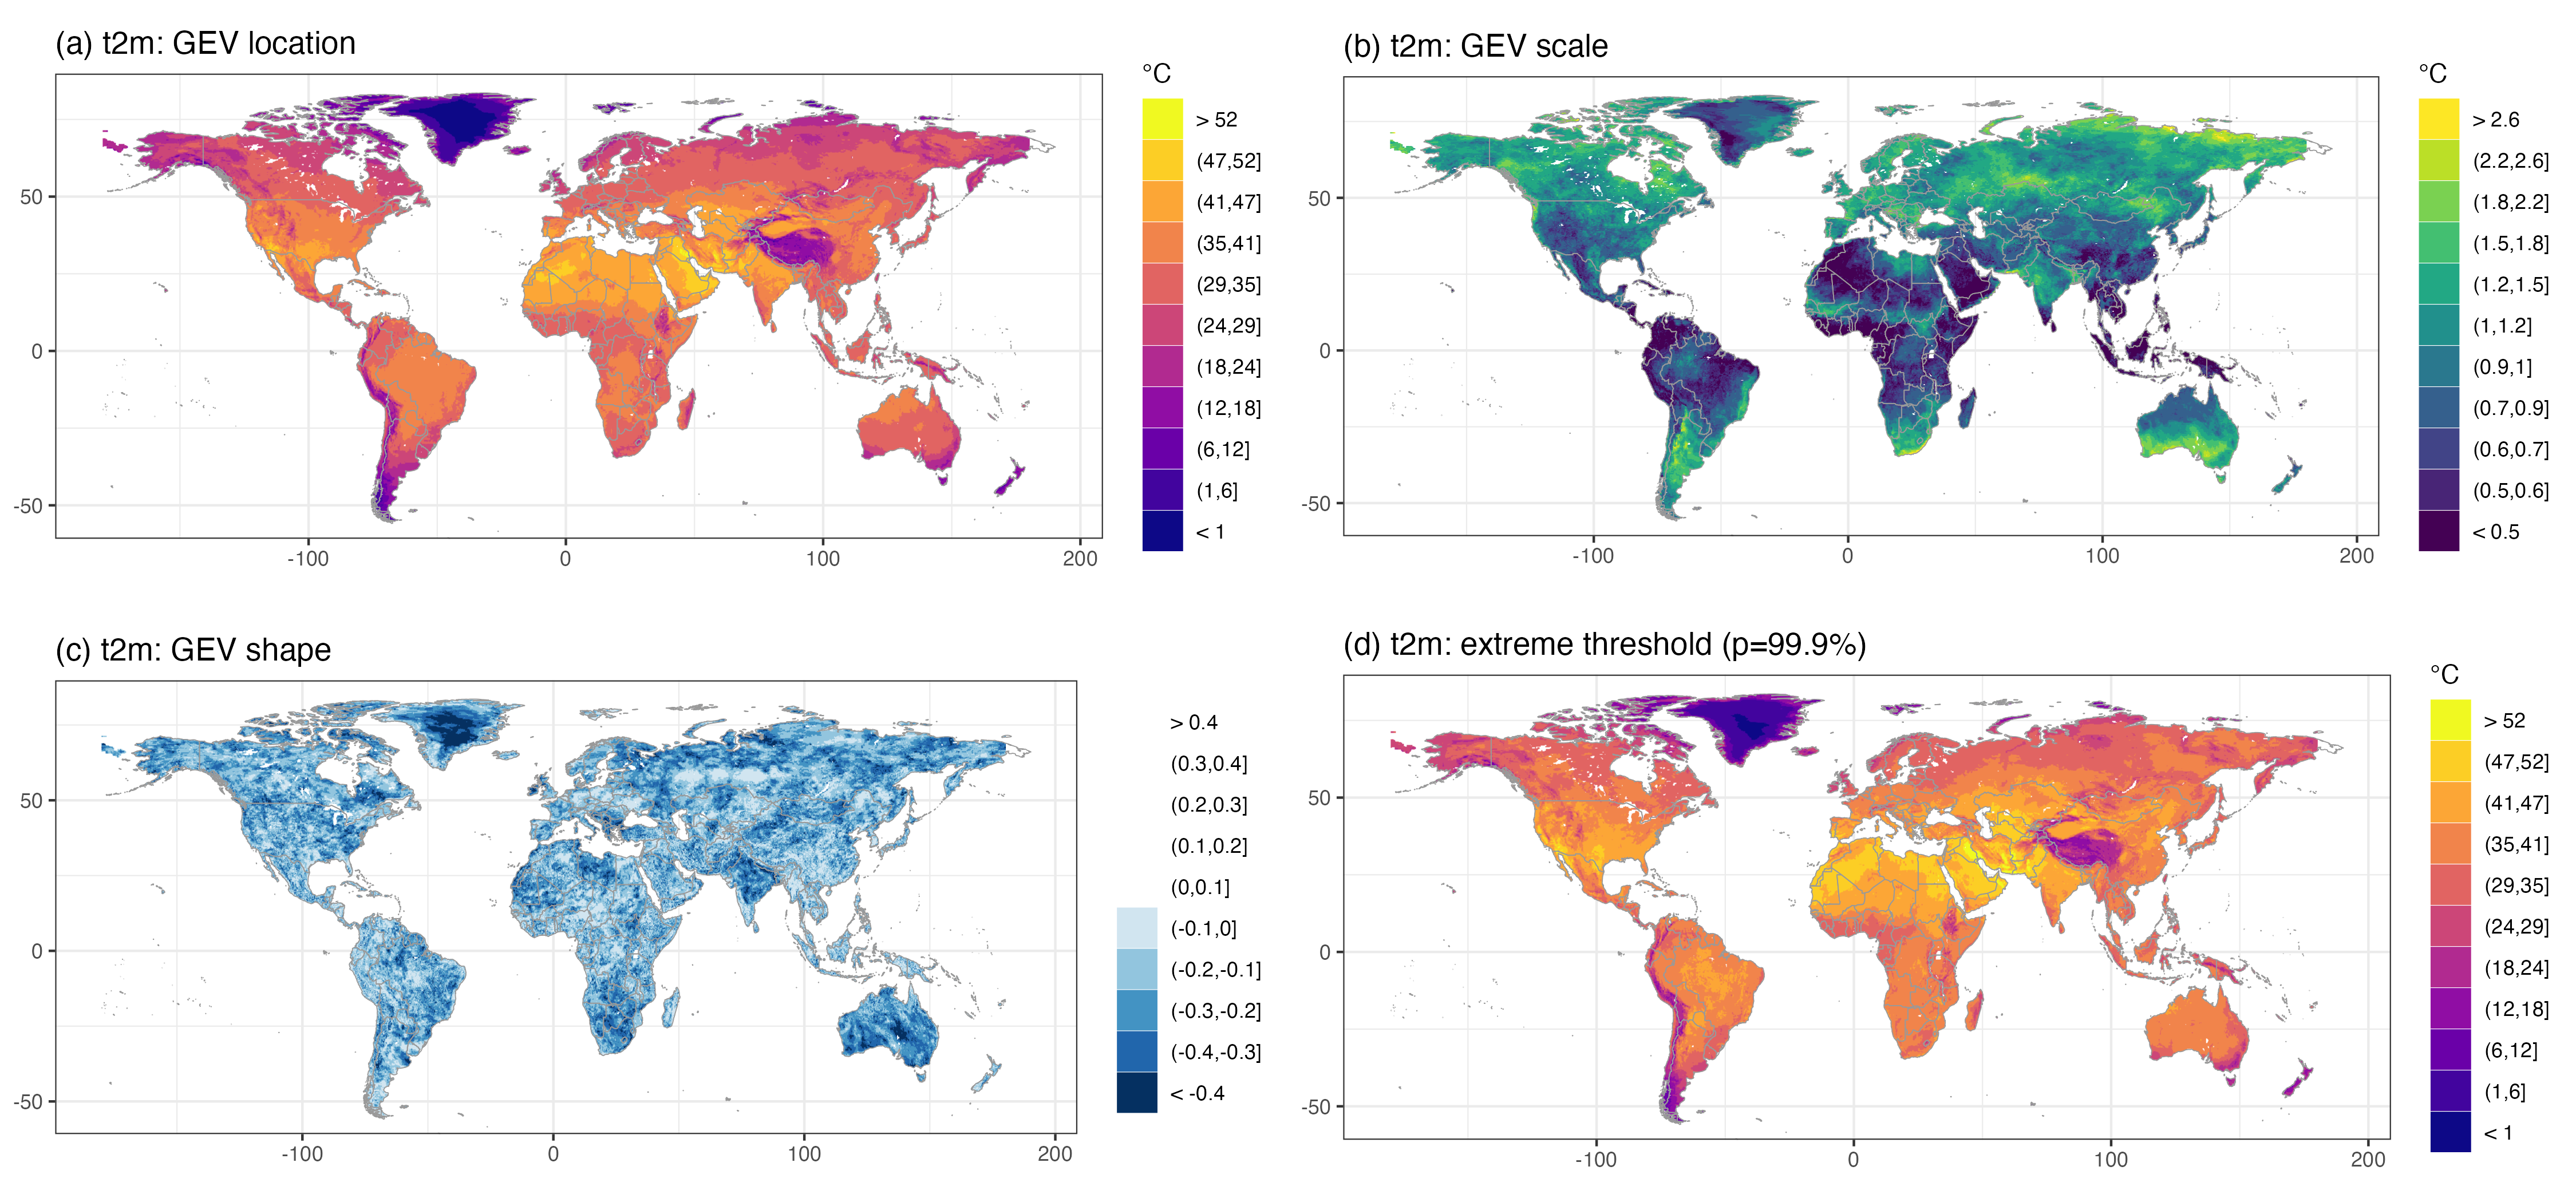
\includegraphics[width=\textwidth]{Figure_GEVfields_t2m_gridbox.png}
    \caption{Best estimates (posterior medians) of the IFS-GEV fields and extreme thresholds for 2m temperature.}
    \label{fig:bestGEVt2m}
\end{figure}

\begin{figure}[!t]
    \centering
    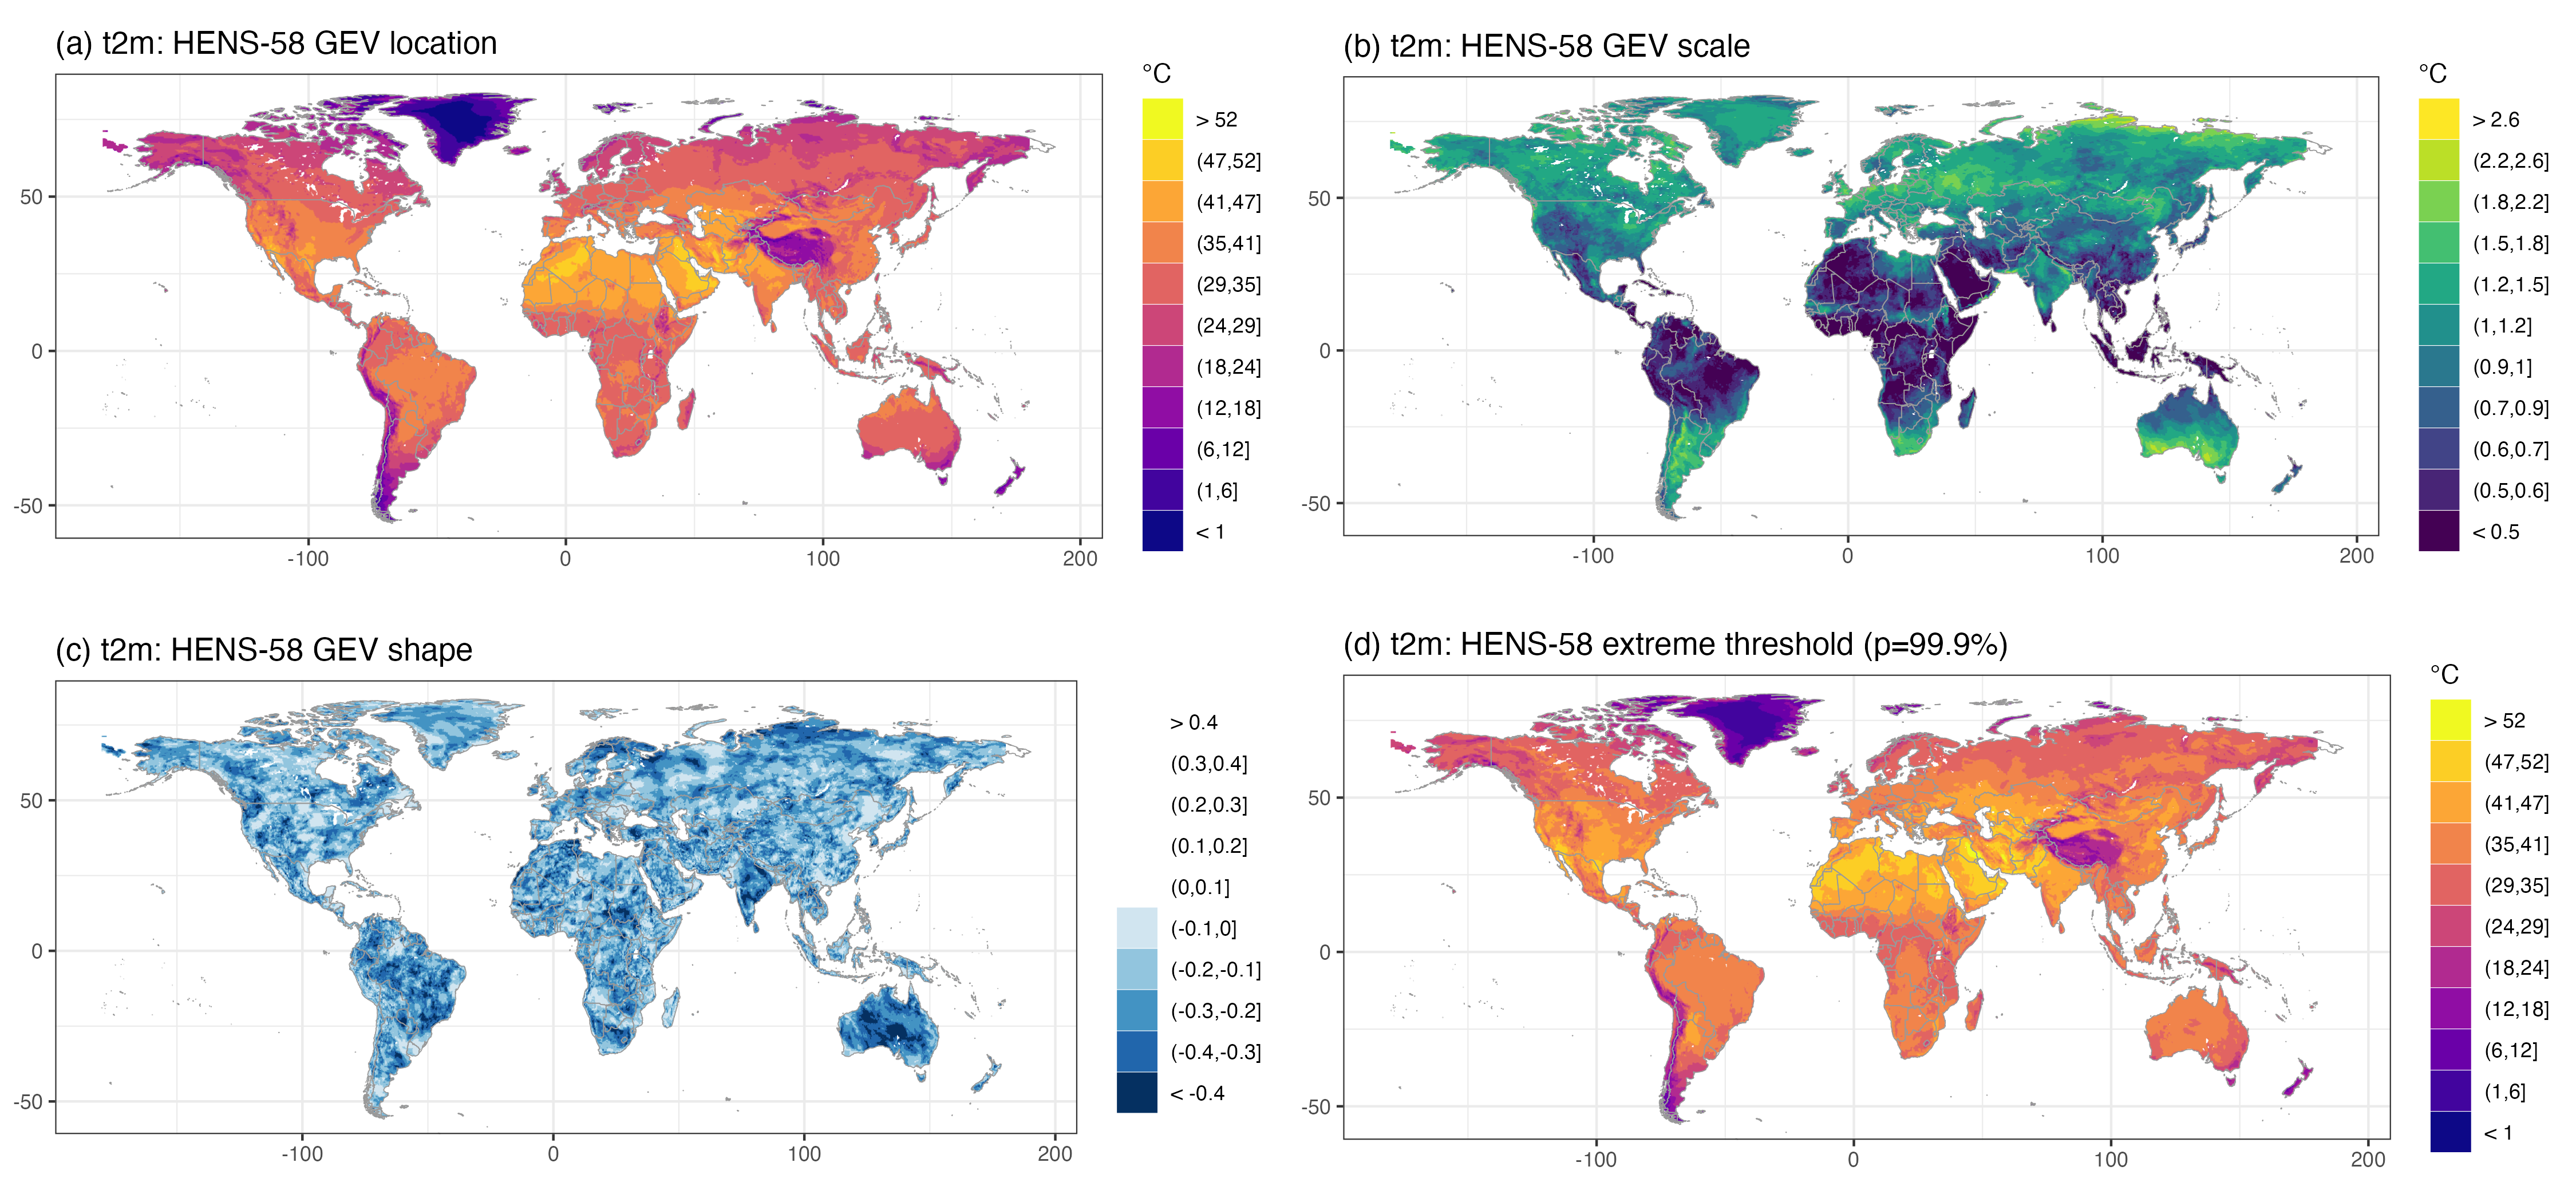
\includegraphics[width=\textwidth]{Figure_GEVfields_t2m_HENS58_gridbox.png}
    \caption{Best estimates (posterior medians) of the HENS-58-GEV fields and extreme thresholds for 2m temperature.}
    \label{fig:bestGEVt2m_HENS58}
\end{figure}

\begin{figure}[!t]
    \centering
    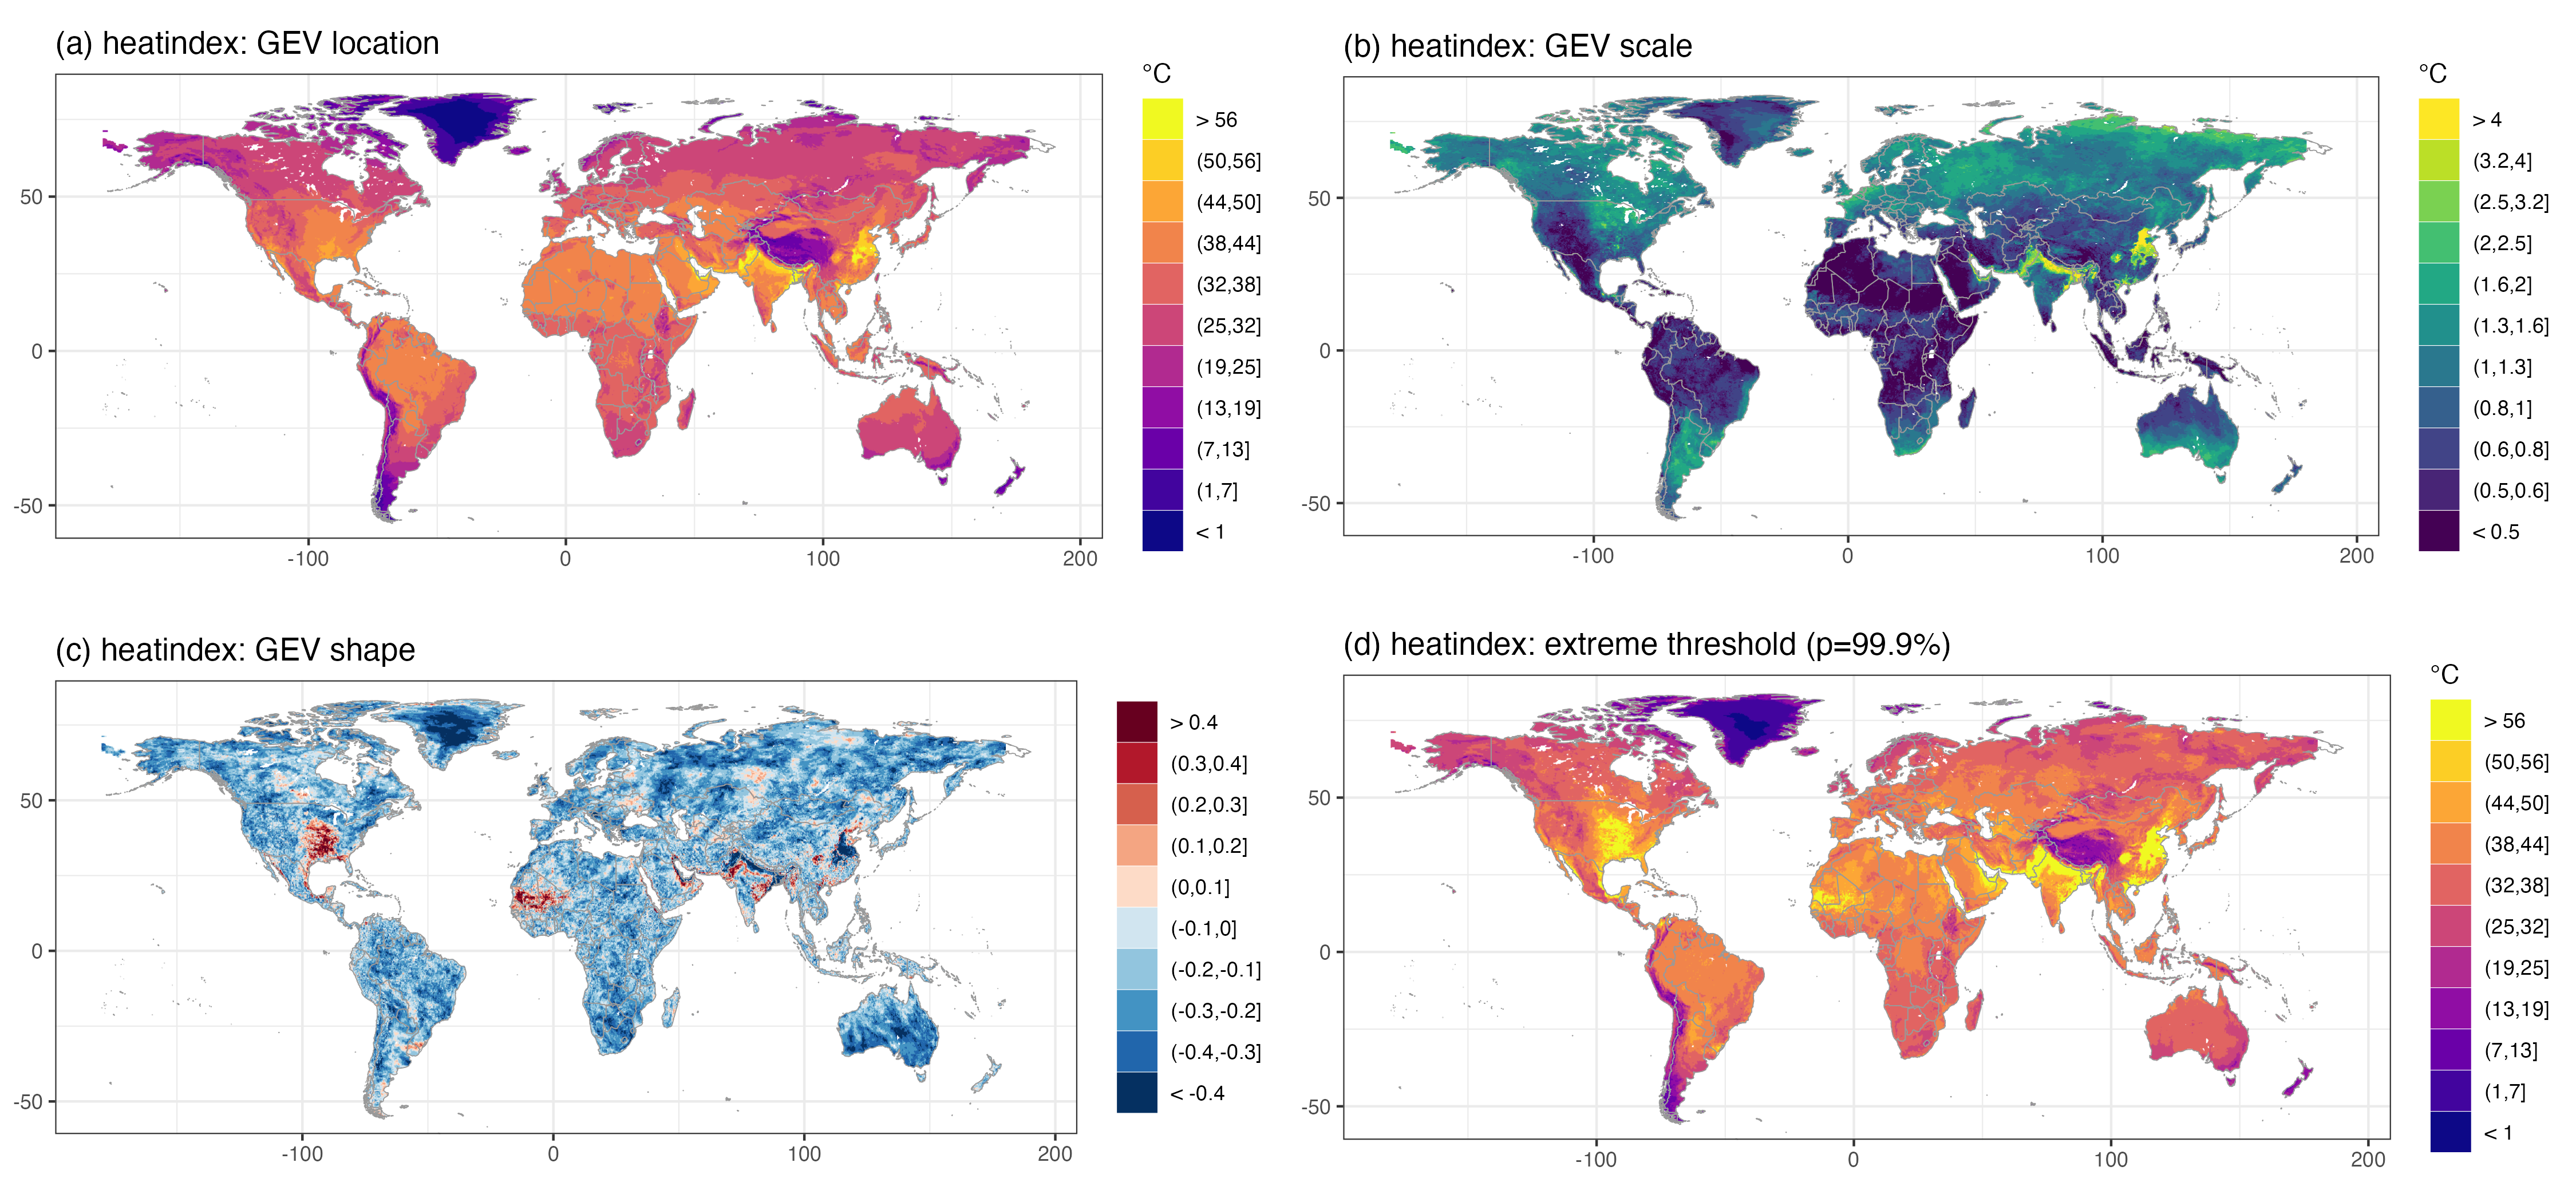
\includegraphics[width=\textwidth]{Figure_GEVfields_heatindex_gridbox.png}
    \caption{Best estimates (posterior medians) of the IFS-GEV fields and extreme thresholds for the heat index.}
    \label{fig:bestGEVheatindex}
\end{figure}

\begin{figure}[!t]
    \centering
    \includegraphics[width=\textwidth]{Figure_GEVfields_heatindex_HENS58_gridbox.png}
    \caption{Best estimates (posterior medians) of the HENS-58-GEV fields and extreme thresholds for the heat index.}
    \label{fig:bestGEVheatindex_HENS58}
\end{figure}


\color{red}
\newpage

\subsection{Testing GEV assumptions}

The fundamental challenge in modeling the far upper tail and whether a statistical model can adequately represent the behavior of unobserved extremes beyond the support of the data rests in determining whether the underlying postulates under which the distribution of block maxima may converge to the GEV distribution hold in nature. It is therefore critical to ensure that the GEV assumptions are reasonably satisfied (i.e., that the GEV distribution provides a suitable fit to the data) by the statistical model described in Section~\ref{sec_global}. This is a challenging task given the large number of grid boxes across two ensembles and two output variables.

One approach for checking the goodness of fit for a statistical distribution to an empirical sample is via a quantile-quantile (Q-Q) plot, which compares the sample quantiles of the data with the corresponding ``theoretical'' quantiles of the fitted distribution. Points falling along the 45$^\circ$ (1-1) line are evidence of a good fit, i.e., that the sample quantiles are equal to the theoretical quantiles. The goodness of fit should of course be relative to the statistical uncertainty, which is accounted for with a pointwise method based on the Kolmogorov-Smirnov distribution \citep{Owen1995}. For each grid box, variable, and ensemble, we  compare the maxima against the theoretical quantiles of a $\text{GEV}(\mu,\sigma,\xi)$ distribution, using the posterior mean estimates of the GEV coefficients. To summarize the large number of gauged locations, we then simply count the number of measurements that fall outside the 95\% confidence band of the Q-Q plot, stratifying by the upper and lower tail. Anything less than 5\% of all points indicates that the GEV distribution provides a good fit to the data, and hence the GEV assumptions are satisfied.


\begin{figure}[!t]
    \centering
    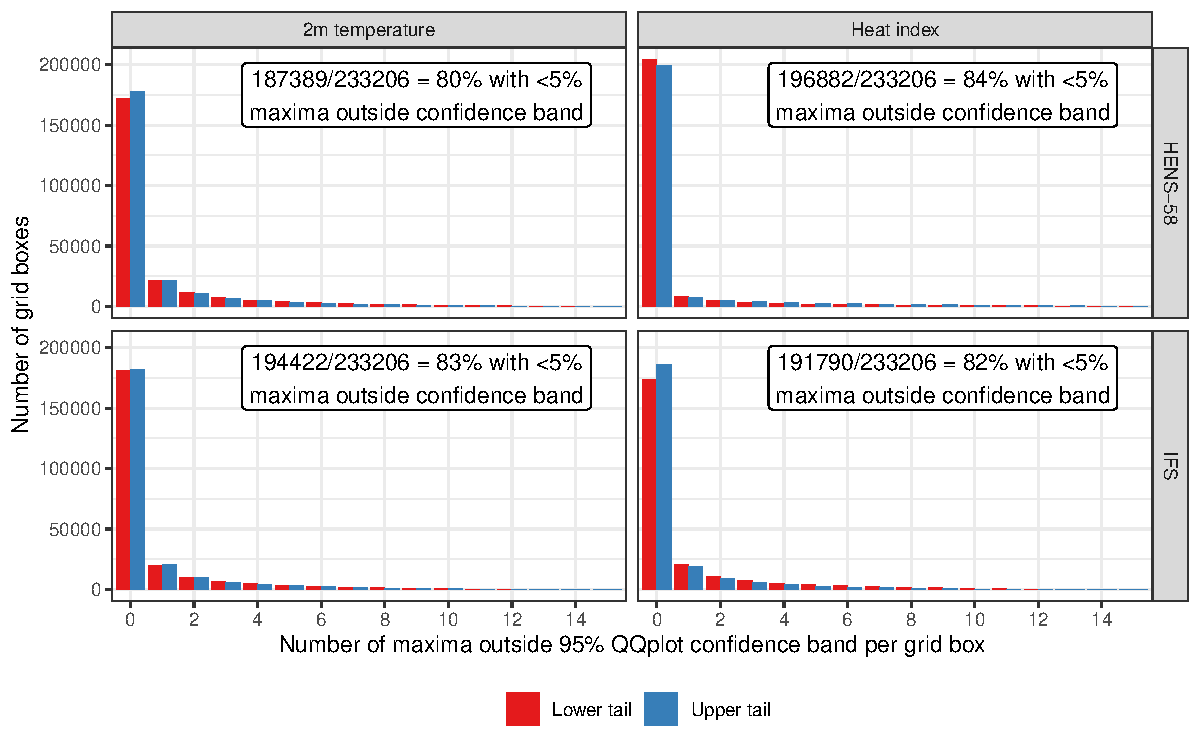
\includegraphics[width=\textwidth]{Figure_outsideCI_QQplots.pdf}
    \caption{Tally of the number of extreme measurements that fall outside the 95\% confidence band for the heat index and 2m temperatures in the IFS and HENS-58 ensemble. Fewer than 5\% of points (less than 3 out of 50 and 58 ensemble members, respectively) indicates a good statistical fit for the inferred GEV distribution.}
    \label{fig:qq_agg}
\end{figure}

Results are shown in Figure~\ref{fig:qq_agg}. The GEV distributions from both ensembles and variables provide an excellent fit to a large majority of the data: more than 80\% of grid boxes have less than 5\% of points falling outside the confidence band. These results provide strong evidence that the GEV assumptions are satisfied and we can be confident in using the fitted distributions to assess the extreme upper tail behavior.

\subsection{Comparing IFS-GEV with HENS-58-GEV}

A simple comparison of the GEV fields obtained from IFS and HENS-58 can be conducted by looking at the difference in posteriors from each statistical fit. Best estimates of this difference are calculated as the difference in posterior means. To account for the uncertainty innate to fitting GEV distributions to a finite sample, we then calculate a 95\% credible interval for the difference and use stippling to denote where the uncertainty interval includes zero. 

\begin{figure}[!t]
    \centering
    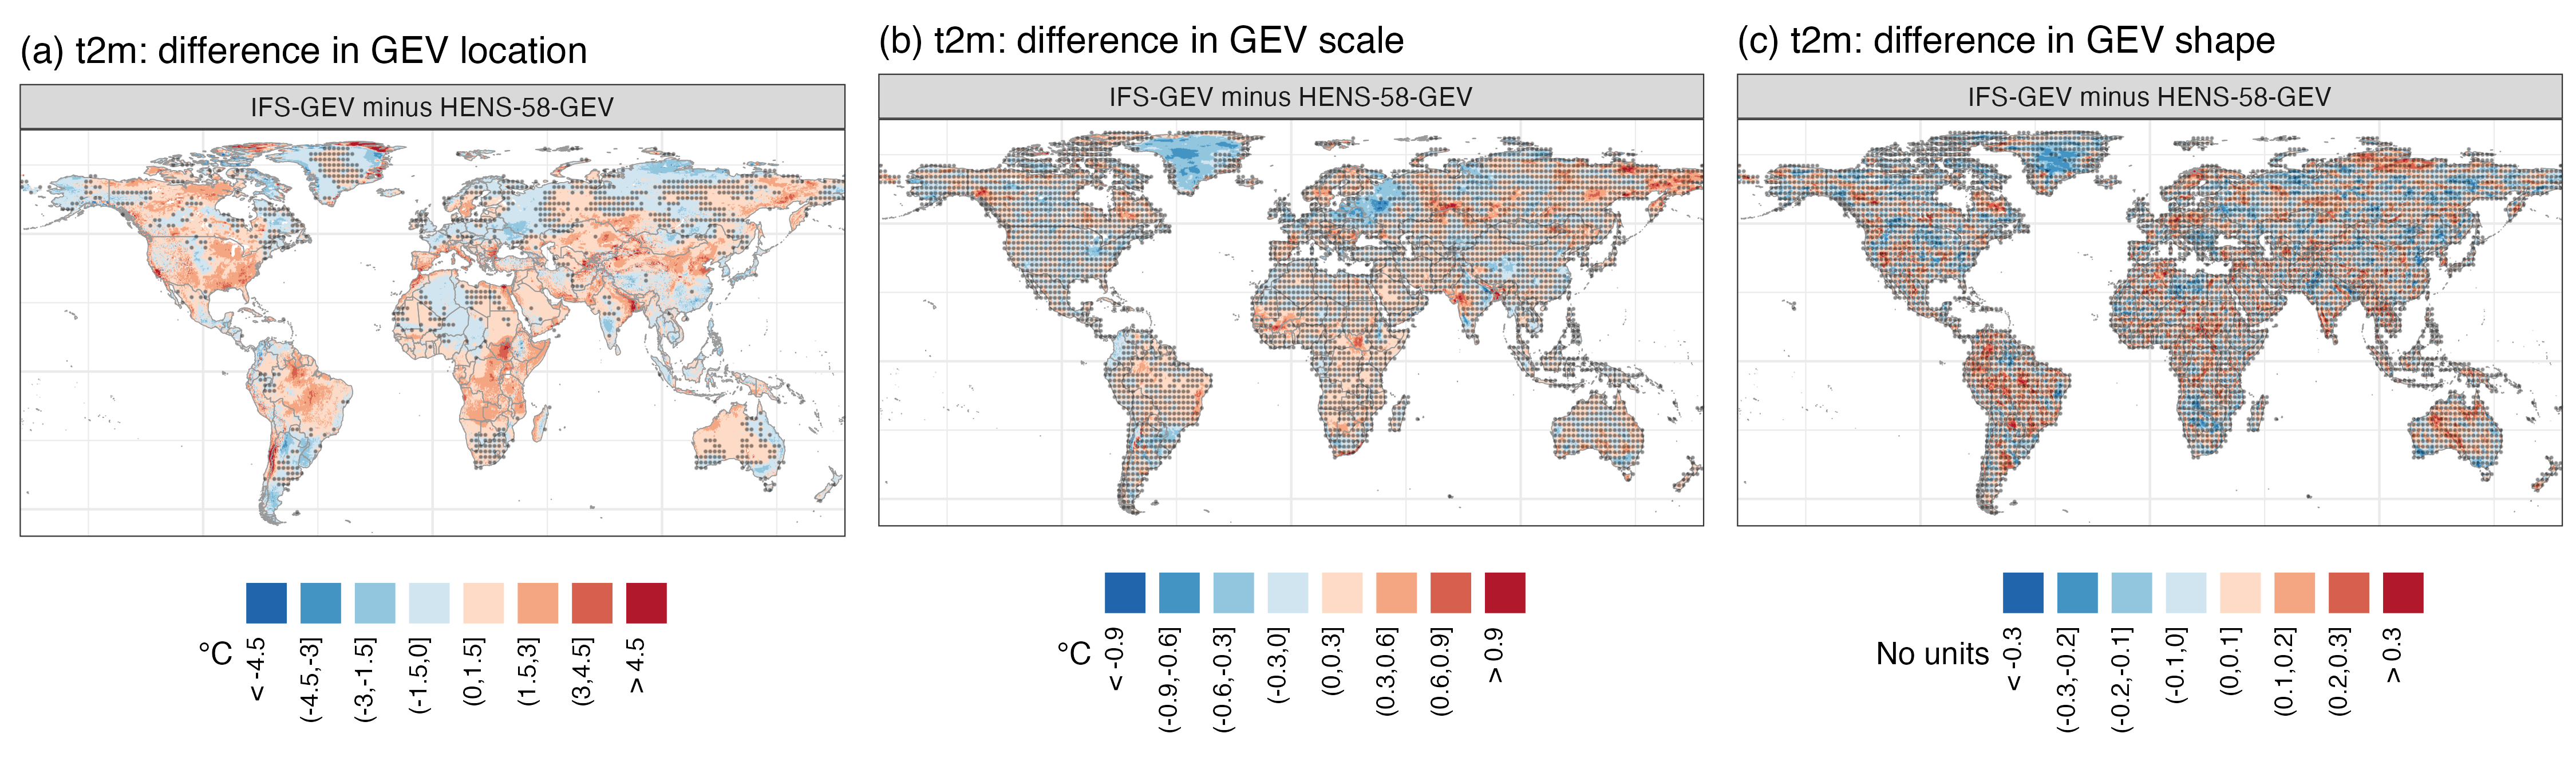
\includegraphics[width=\textwidth]{Figure_GEVfields_t2m_IFS_vs_HENS58_diff.png}
    \caption{Best estimates (posterior means) of the difference between IFS-GEV and HENS-58-GEV fields for t2m. Stippling denotes where this difference is \textit{not} significant (the 95\% uncertainty interval includes zero).}
    \label{fig:GEVdiff}
\end{figure}

Results for 2m temperatures are shown in Figure~\ref{fig:GEVdiff}. The GEV location fields from both ensembles are quite different, with the IFS-GEV location larger than the HENS-58-GEV location for most of the globe. Interestingly, the spatial pattern of Figure~\ref{fig:GEVdiff}(a) aligns quite closely with the difference in ensemble maxima shown in Figure 1(b) of the main text. Both the GEV scale and shape are statistically indistinguishable in IFS-GEV and HENS-58-GEV for nearly the whole globe. This suggests that both forecast systems yield equivalent performance for resolving the most extreme tail risks for 2m temperatures.


\color{black}

\section{Assessment of HENS realism in Greenland} \label{appdx:greenland}

% \todo{AM 3/6/2026- can we move the Greenland paragraph to supplemental information, for the sake of space and word limits.}
The fact that Greenland stands out so clearly with large anomalies relative to ERA5 in Figure 1 in the main text and \textit{exceptionally unlikely} temperatures relative to IFS-GEV in Figure 2 in thr main text motivates us to examine the realism of emulated temperatures in this region more thoroughly. Figure~\ref{supp:fig:promice2} shows how ERA5, IFS, and HENS data compare with extreme gauge-based two-meter surface temperatures from the  Programme for Monitoring of the Greenland Ice Sheet \cite[PROMICE;][]{Fausto2021,How2022data} database. In 2023, paired comparisons of model grid box with nearest-neighbor PROMICE sites show good agreement between all three data sources and the extreme gauged-based 2m temperatures from PROMICE. The HENS extreme temperature distributions overlap the 2023 PROMICE maxima for 24 of the 32 sites; HENS distributions contain the all-time PROMICE maxima for 29 of 38 sites. Figure~\ref{supp:fig:promice1} summarizes the annual cycle of monthly maximum 2m and surface air temperatures, which shows that the difference between surface and 2m temperatures can exceed 20$^\circ$C in the summer: this is well in line with the 2m air temperatures simulated by HENS. Therefore, we can be confident that HENS is generating realistic high-latitude temperatures in places like Greenland.


\clearpage

\section{Supplemental figures}

\begin{figure*}[!h]
\centering
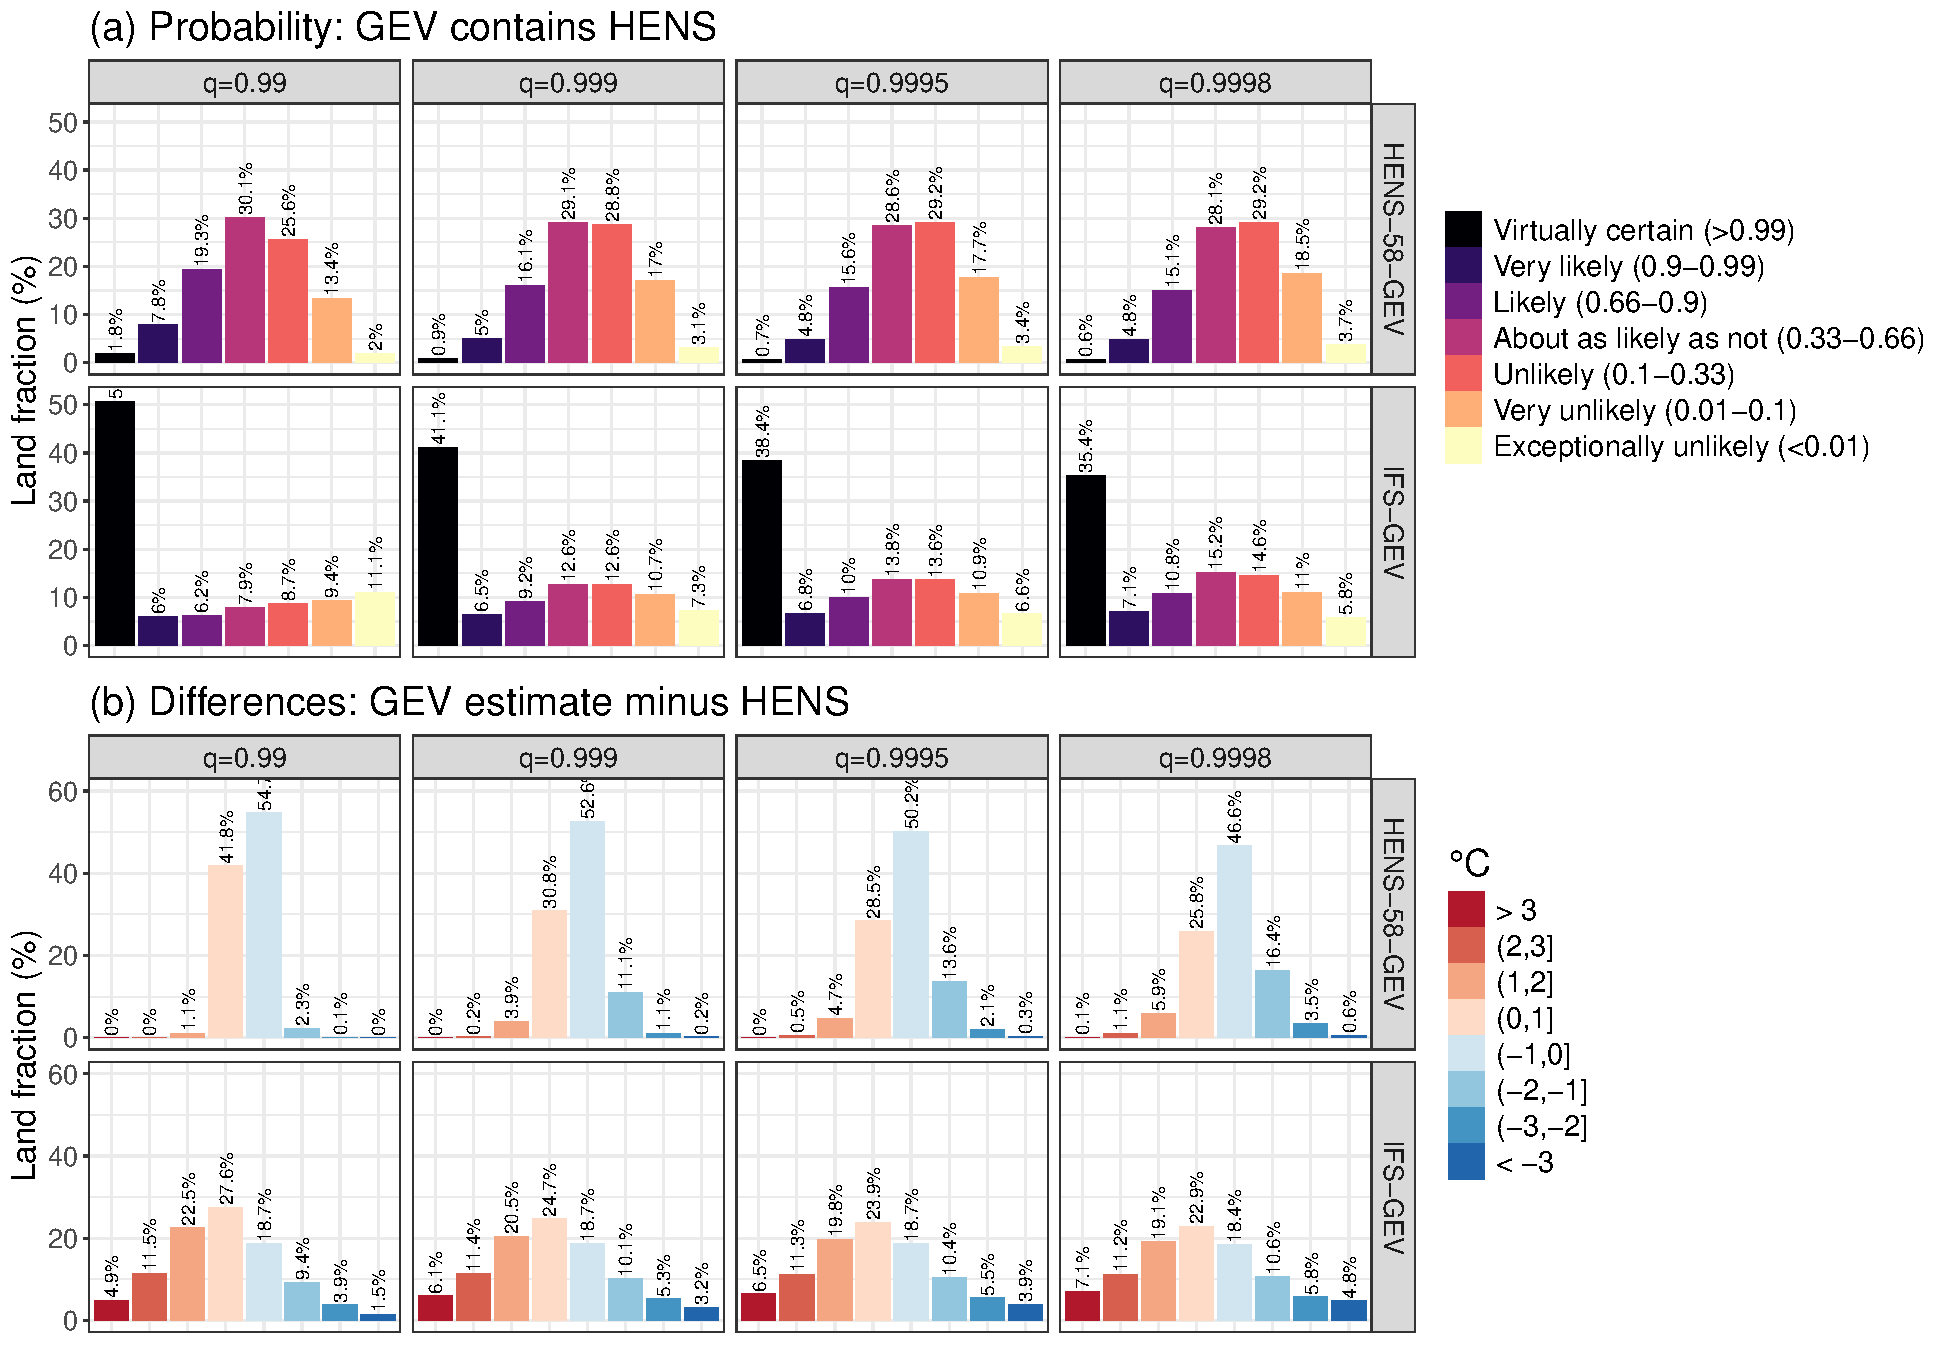
\includegraphics[width = \textwidth]{Figure_t2m_GEV_probContain_HENS_barchart.pdf}
\caption{Tally of the land fraction falling into each category for probability of containment (panel a.) and differences (panel b.) when comparing IFS-GEV, HENS-58-GEV, and HENS return levels. In panel (a), lighter colors indicate that HENS estimates are less likely relative to GEV estimates.}
\label{fig:barchart}
\end{figure*}

\begin{figure}[!h]
    \centering
    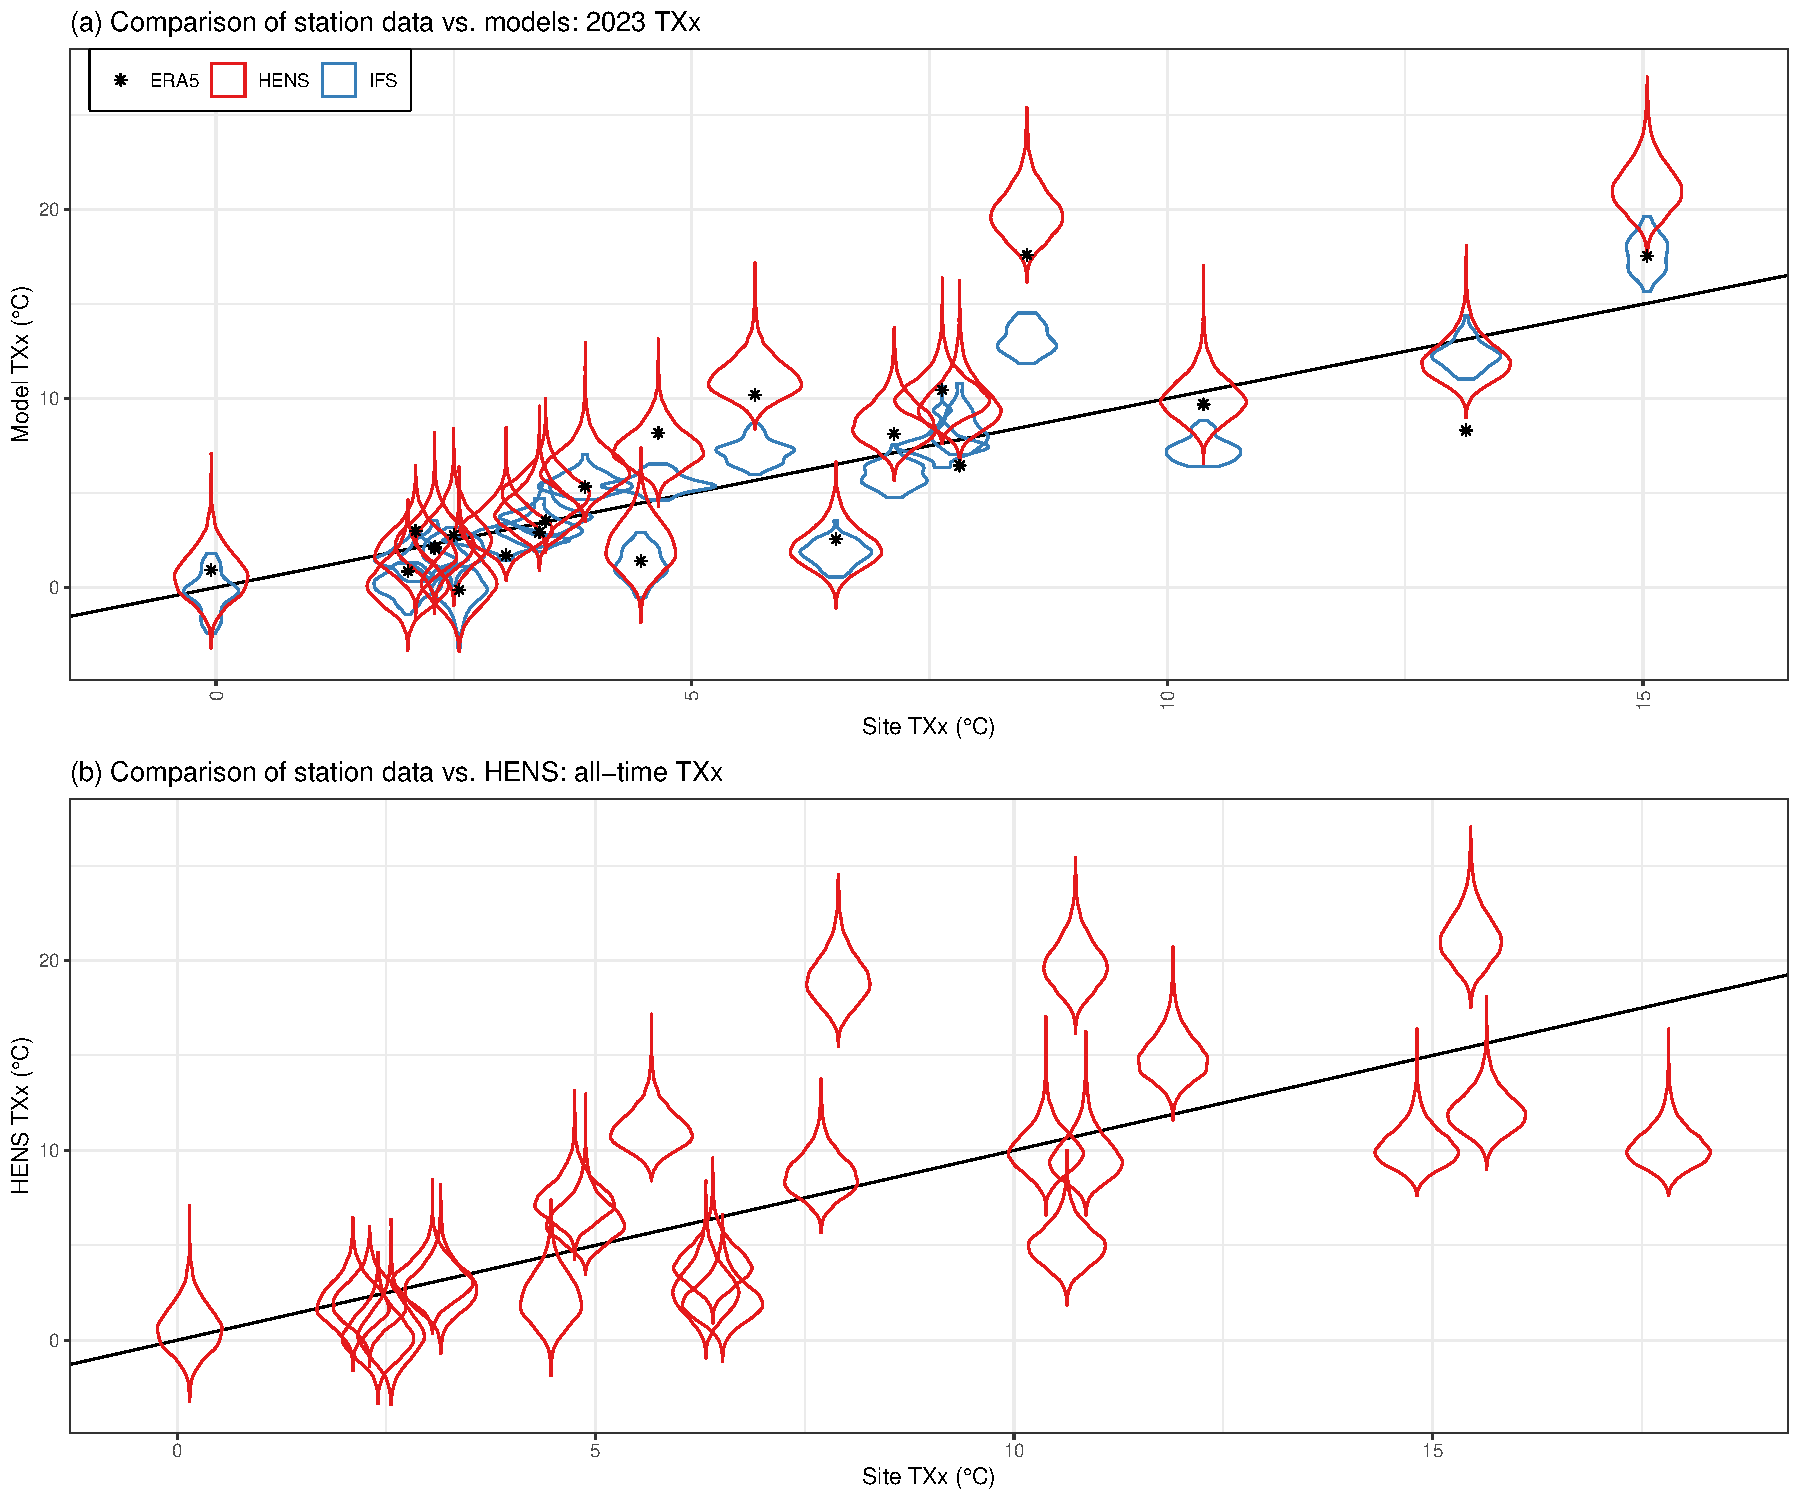
\includegraphics[width=\textwidth]{Figure_PROMICE_vs_Models_v2.pdf}
    \caption{Comparison of the reanalysis and forecast ensemble temperature extremes versus the gauge-based maxima taken from the PROMICE database \citep{Fausto2021,How2022data}, for both 2023 (top) and all-time (bottom).}
    \label{supp:fig:promice2}
\end{figure}

\begin{figure}[!h]
    \centering
    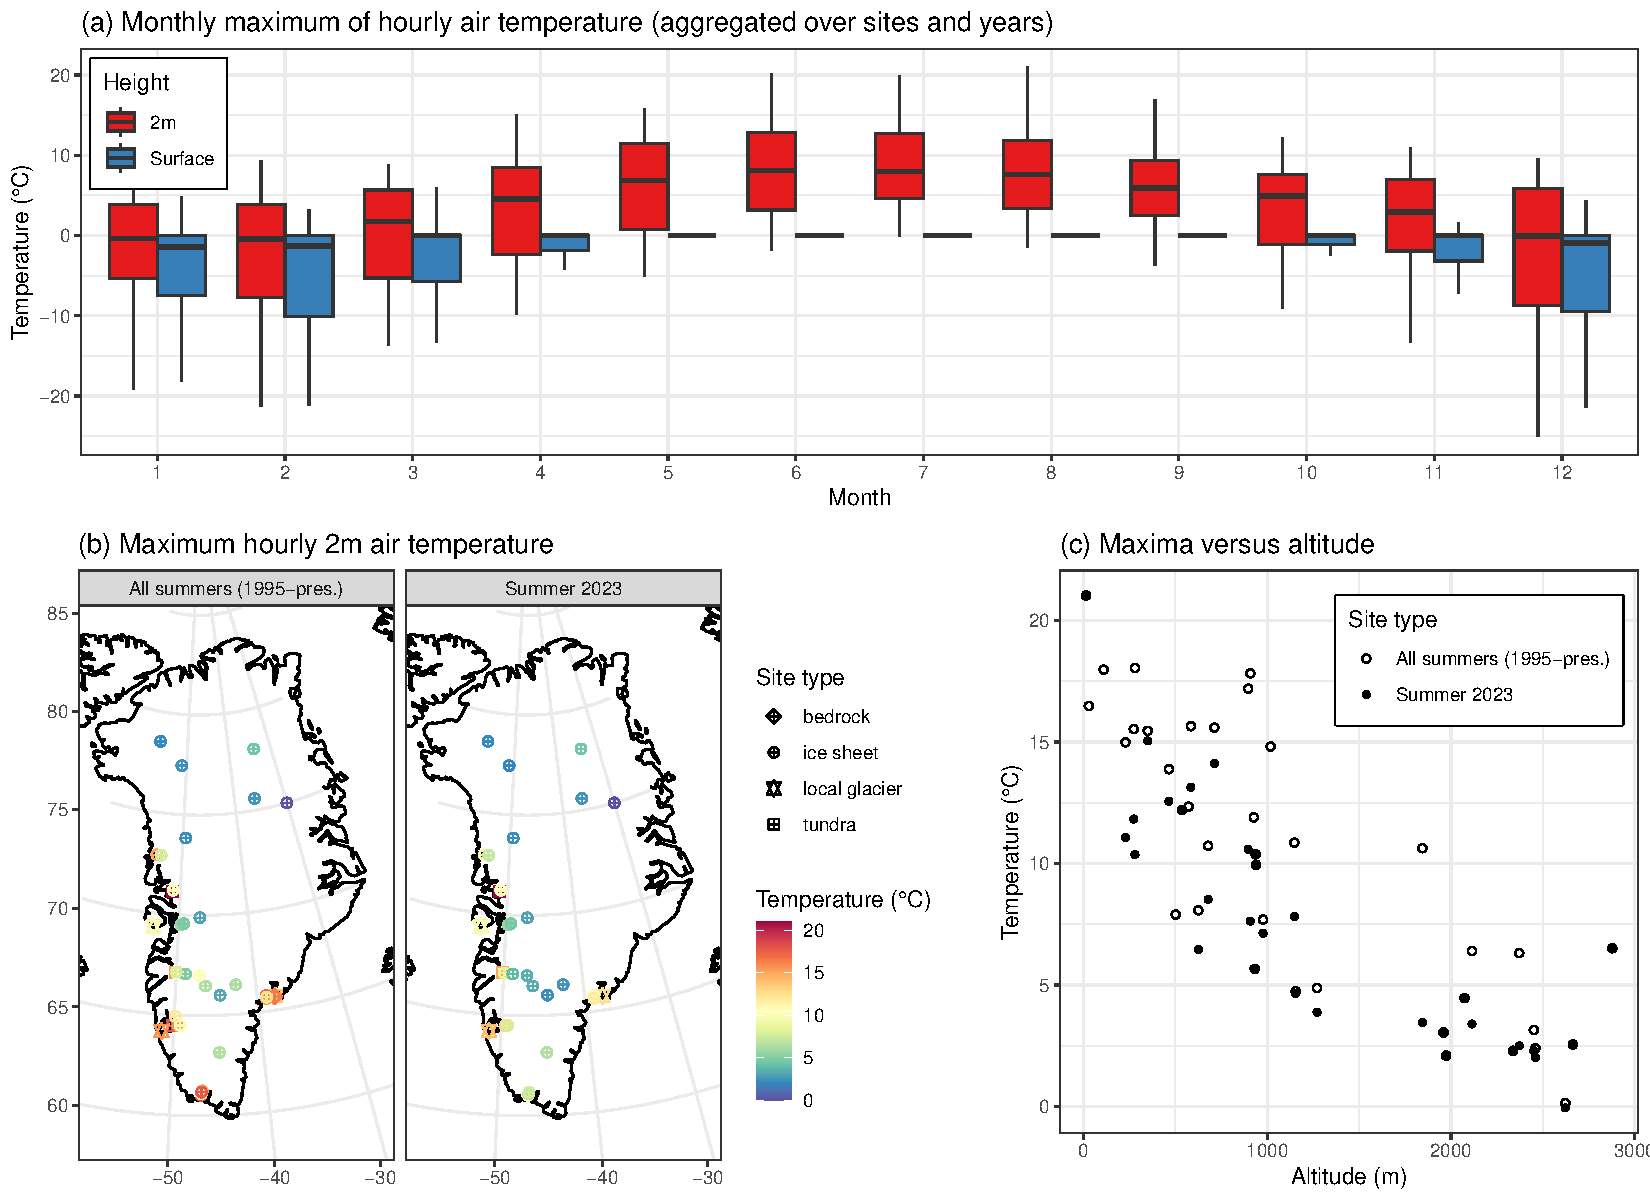
\includegraphics[width=\textwidth]{PROMICE_temperature_extremes_new.pdf}
    \caption{Summary of monthly maximum two-meter air temperature taken from the PROMICE database \citep{Fausto2021,How2022data} over 1995-2024. Panel (a) shows the annual cycle of two-meter vs. surface temperatures, demonstrating that the difference between two-meter and surface temperatures can get as large as 20$^\circ$ in the summer. Panel (b) shows the spatial distribution of the warmest summertime two-meter air temperatures over Greenland, for both the entire record (1995-present) and the 2023 summer. Panel (c) shows how these temperatures depend on elevation. }
    \label{supp:fig:promice1}
\end{figure}



% \begin{figure*}[!t]
% \centering
% 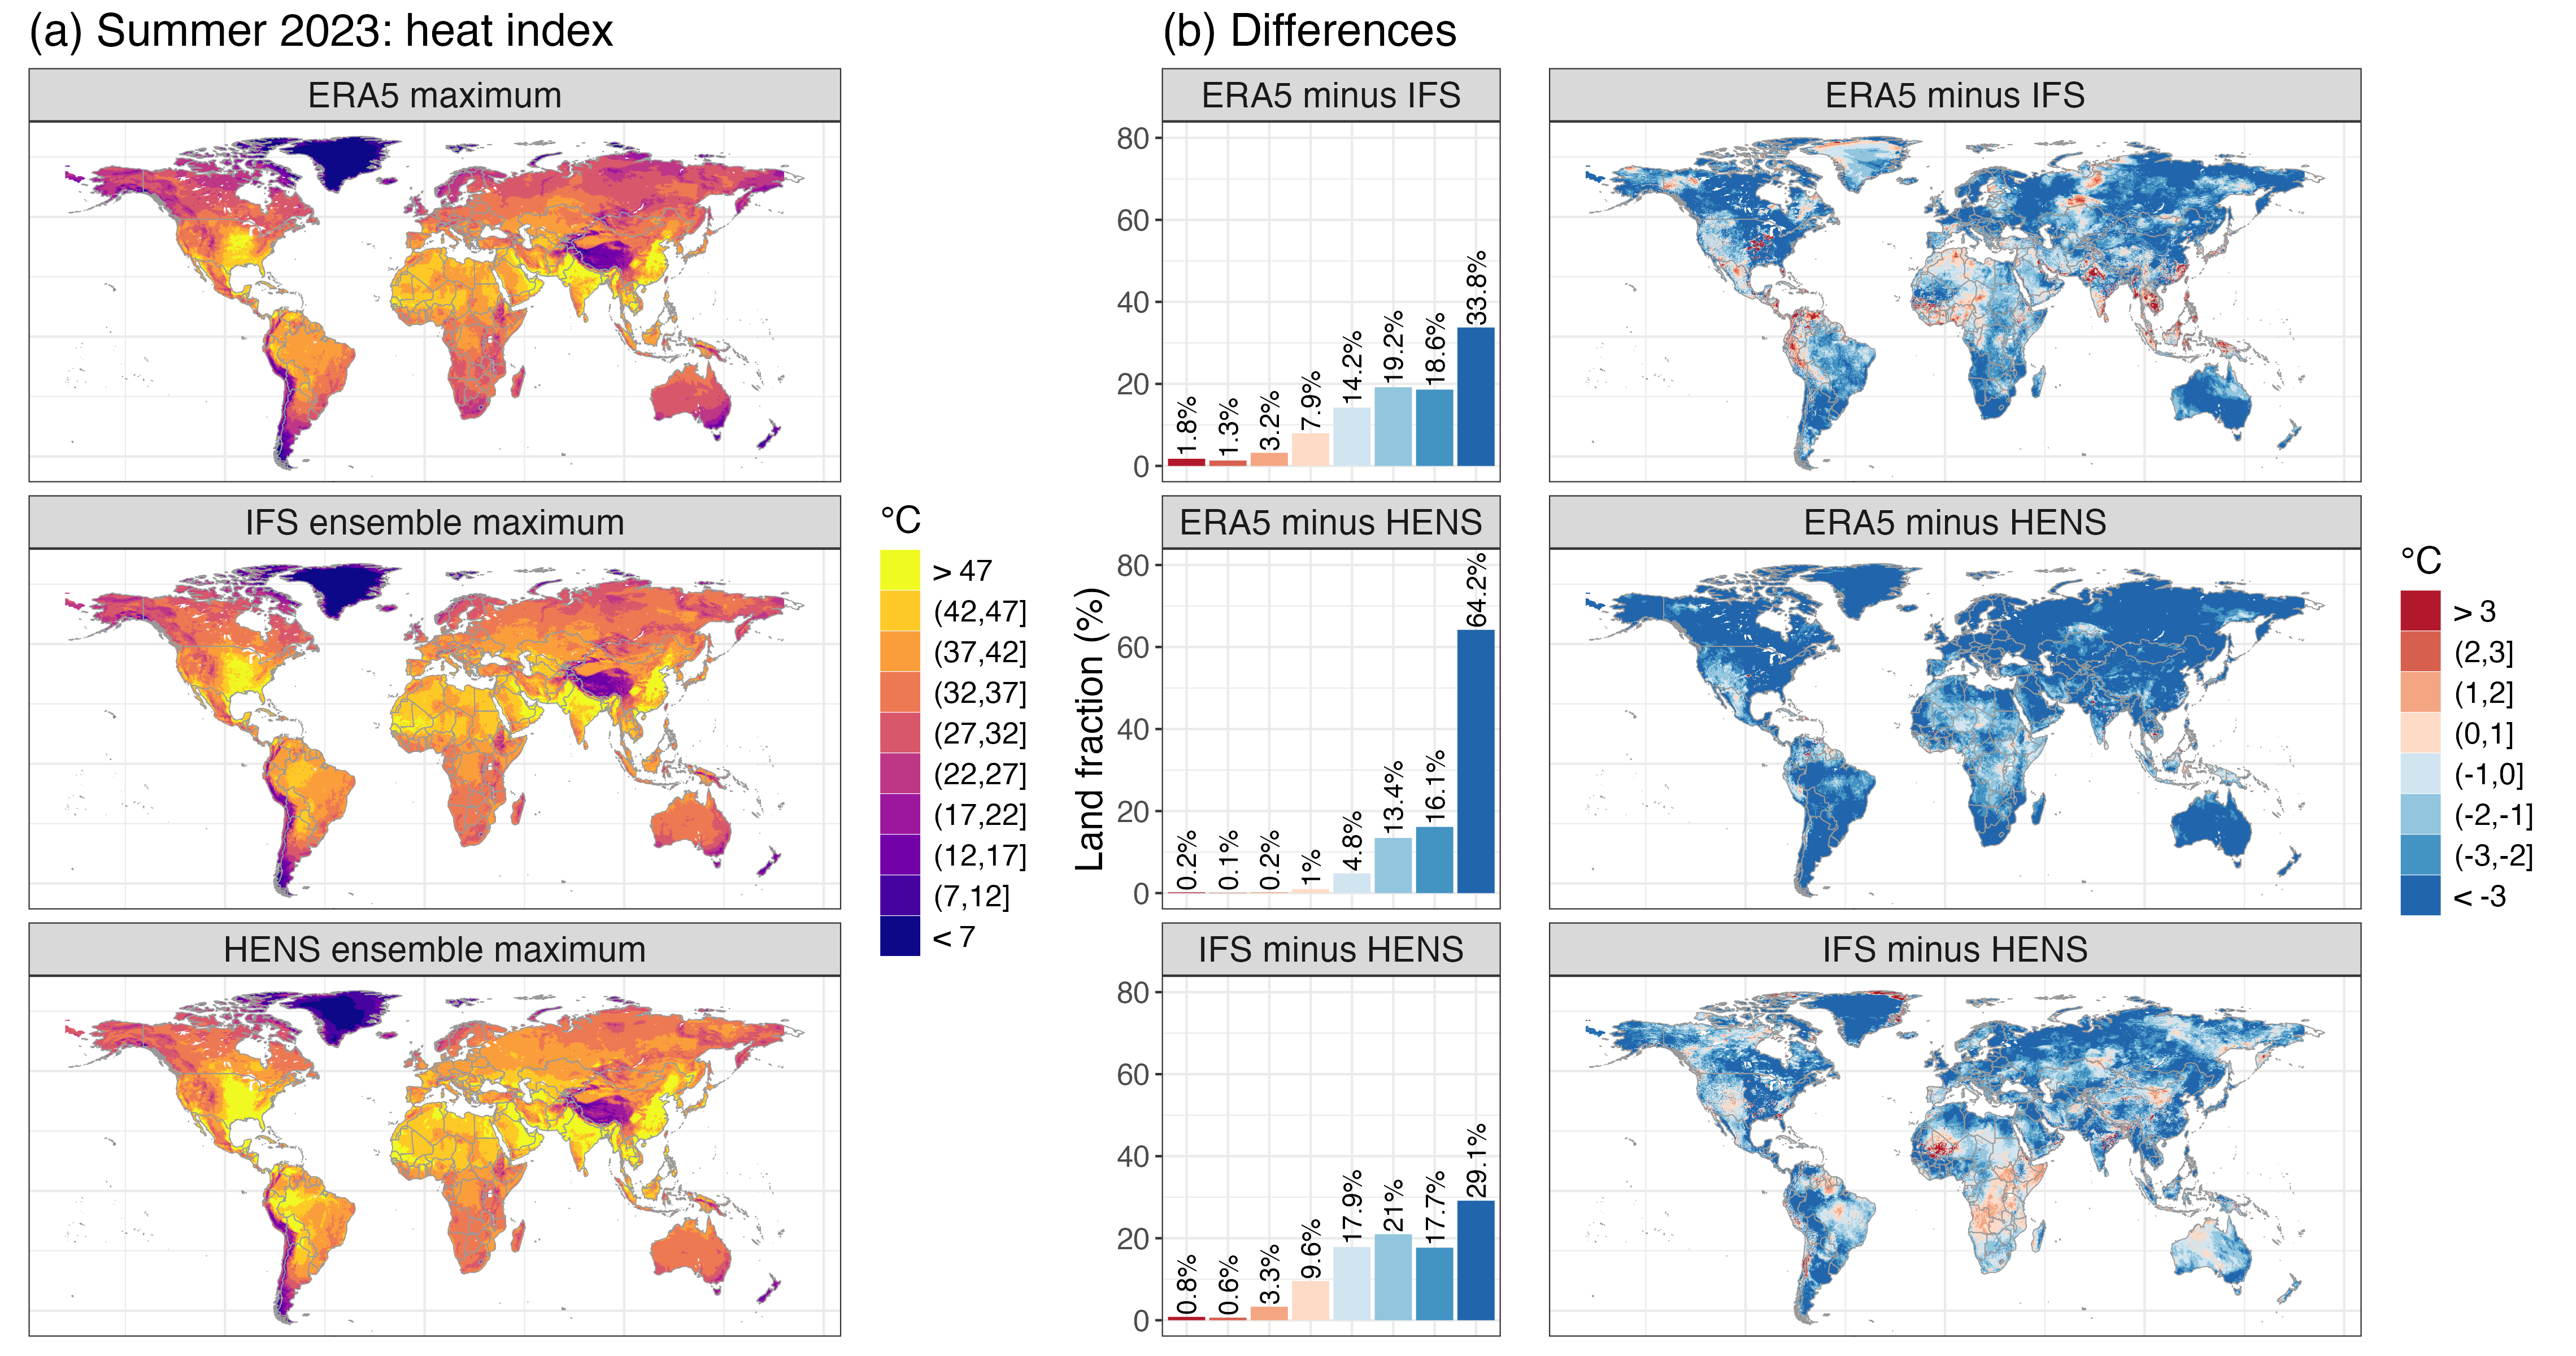
\includegraphics[width = \textwidth]{Figure_heatindex_maxima_diff.png}
% \caption{Comparison of three different versions of the hottest heat index values temperatures over global land regions from 01 June 2023 to 31 August 2023. Panel (a) shows the hottest heat index from ERA5 (our best reconstructions of the realized temperatures; left), the IFS forecast ensemble (middle), and the HENS ensemble (right). Panel (b) compares the differences between three versions of reality.}
% \label{fig:threeversions_hi}
% \end{figure*}


% \begin{figure}
%     \centering
%     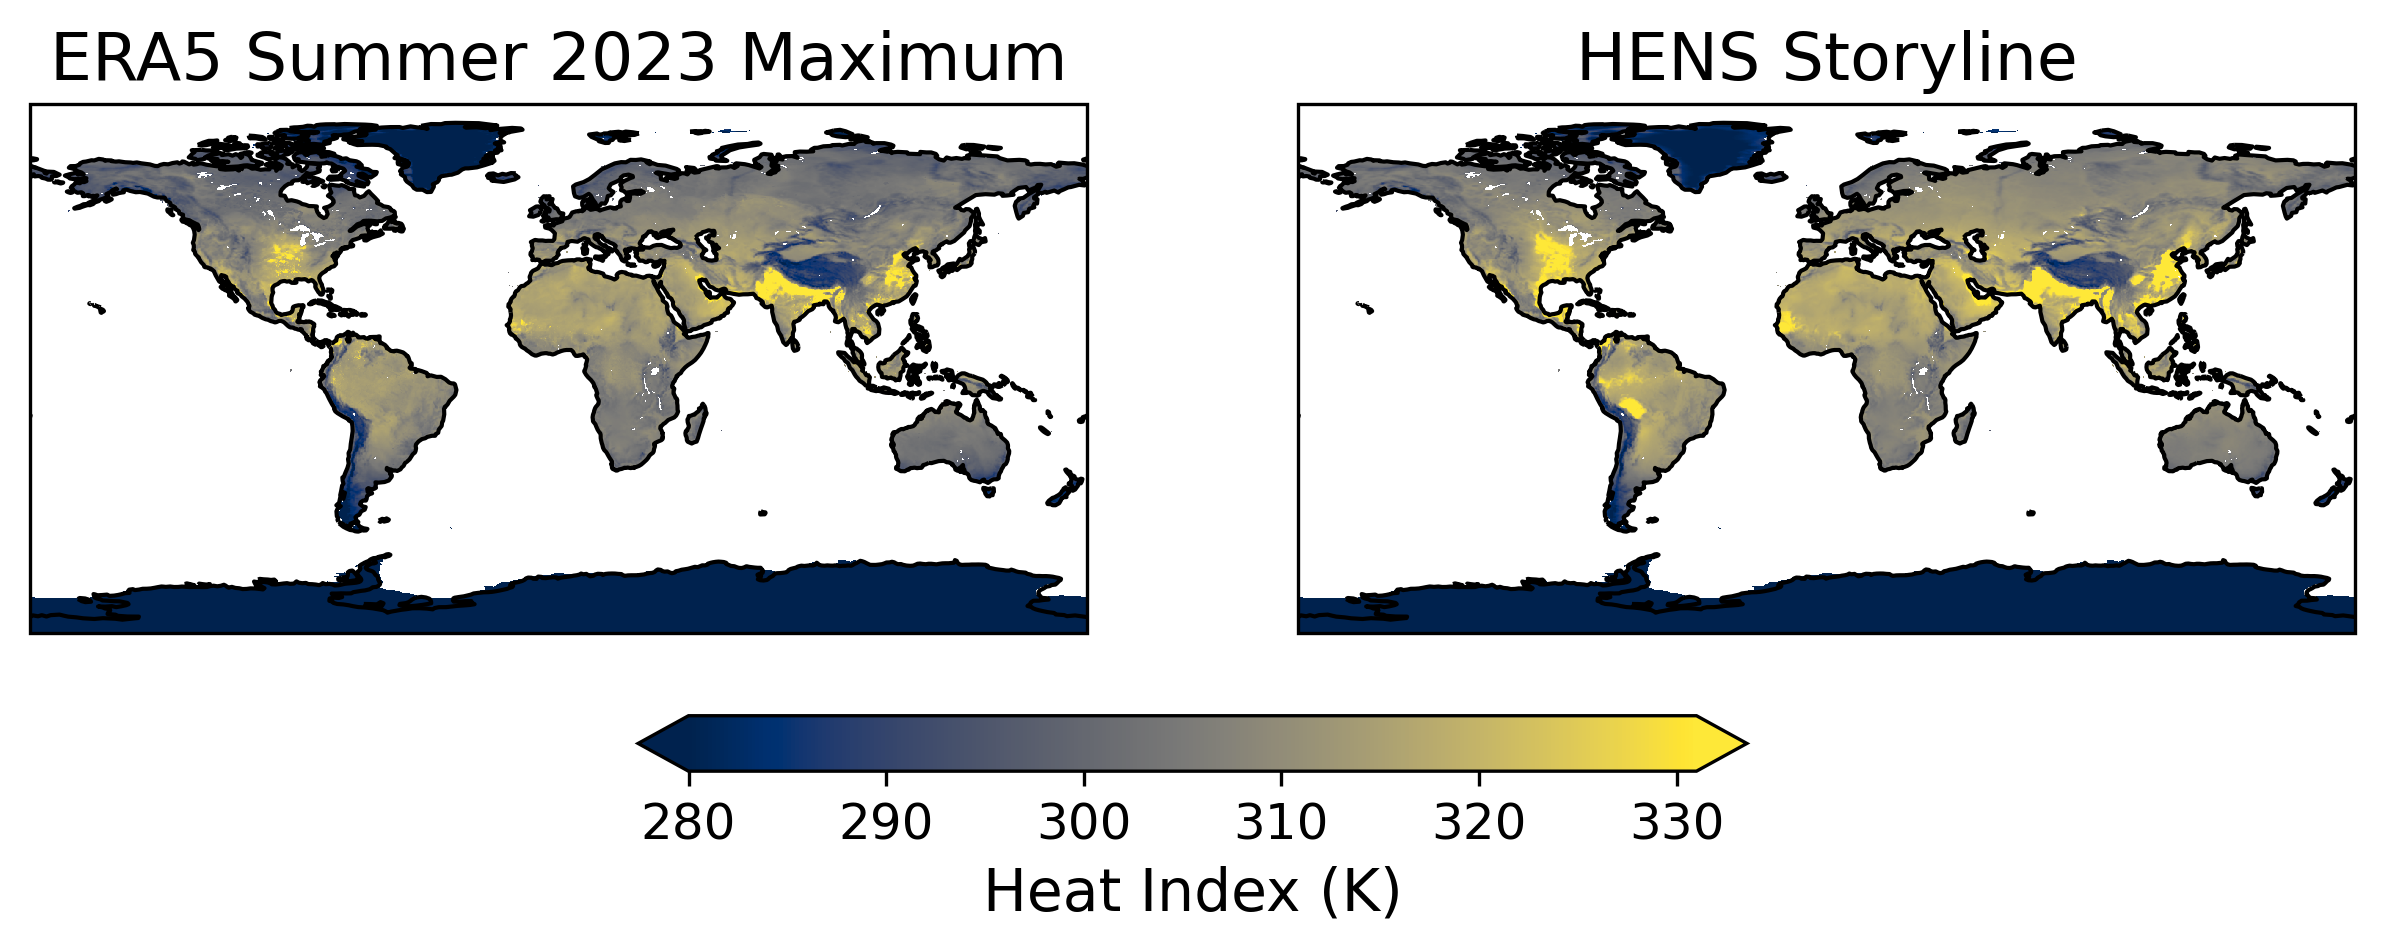
\includegraphics[width=\linewidth]{figures/era5_vs_hens_heatindex.png}
%     \caption{ERA5 vs. HENS Storyline.}
%     \label{fig:era5_vs_hens_storyline_raw}
% \end{figure}

\begin{figure*}[!t]
\centering
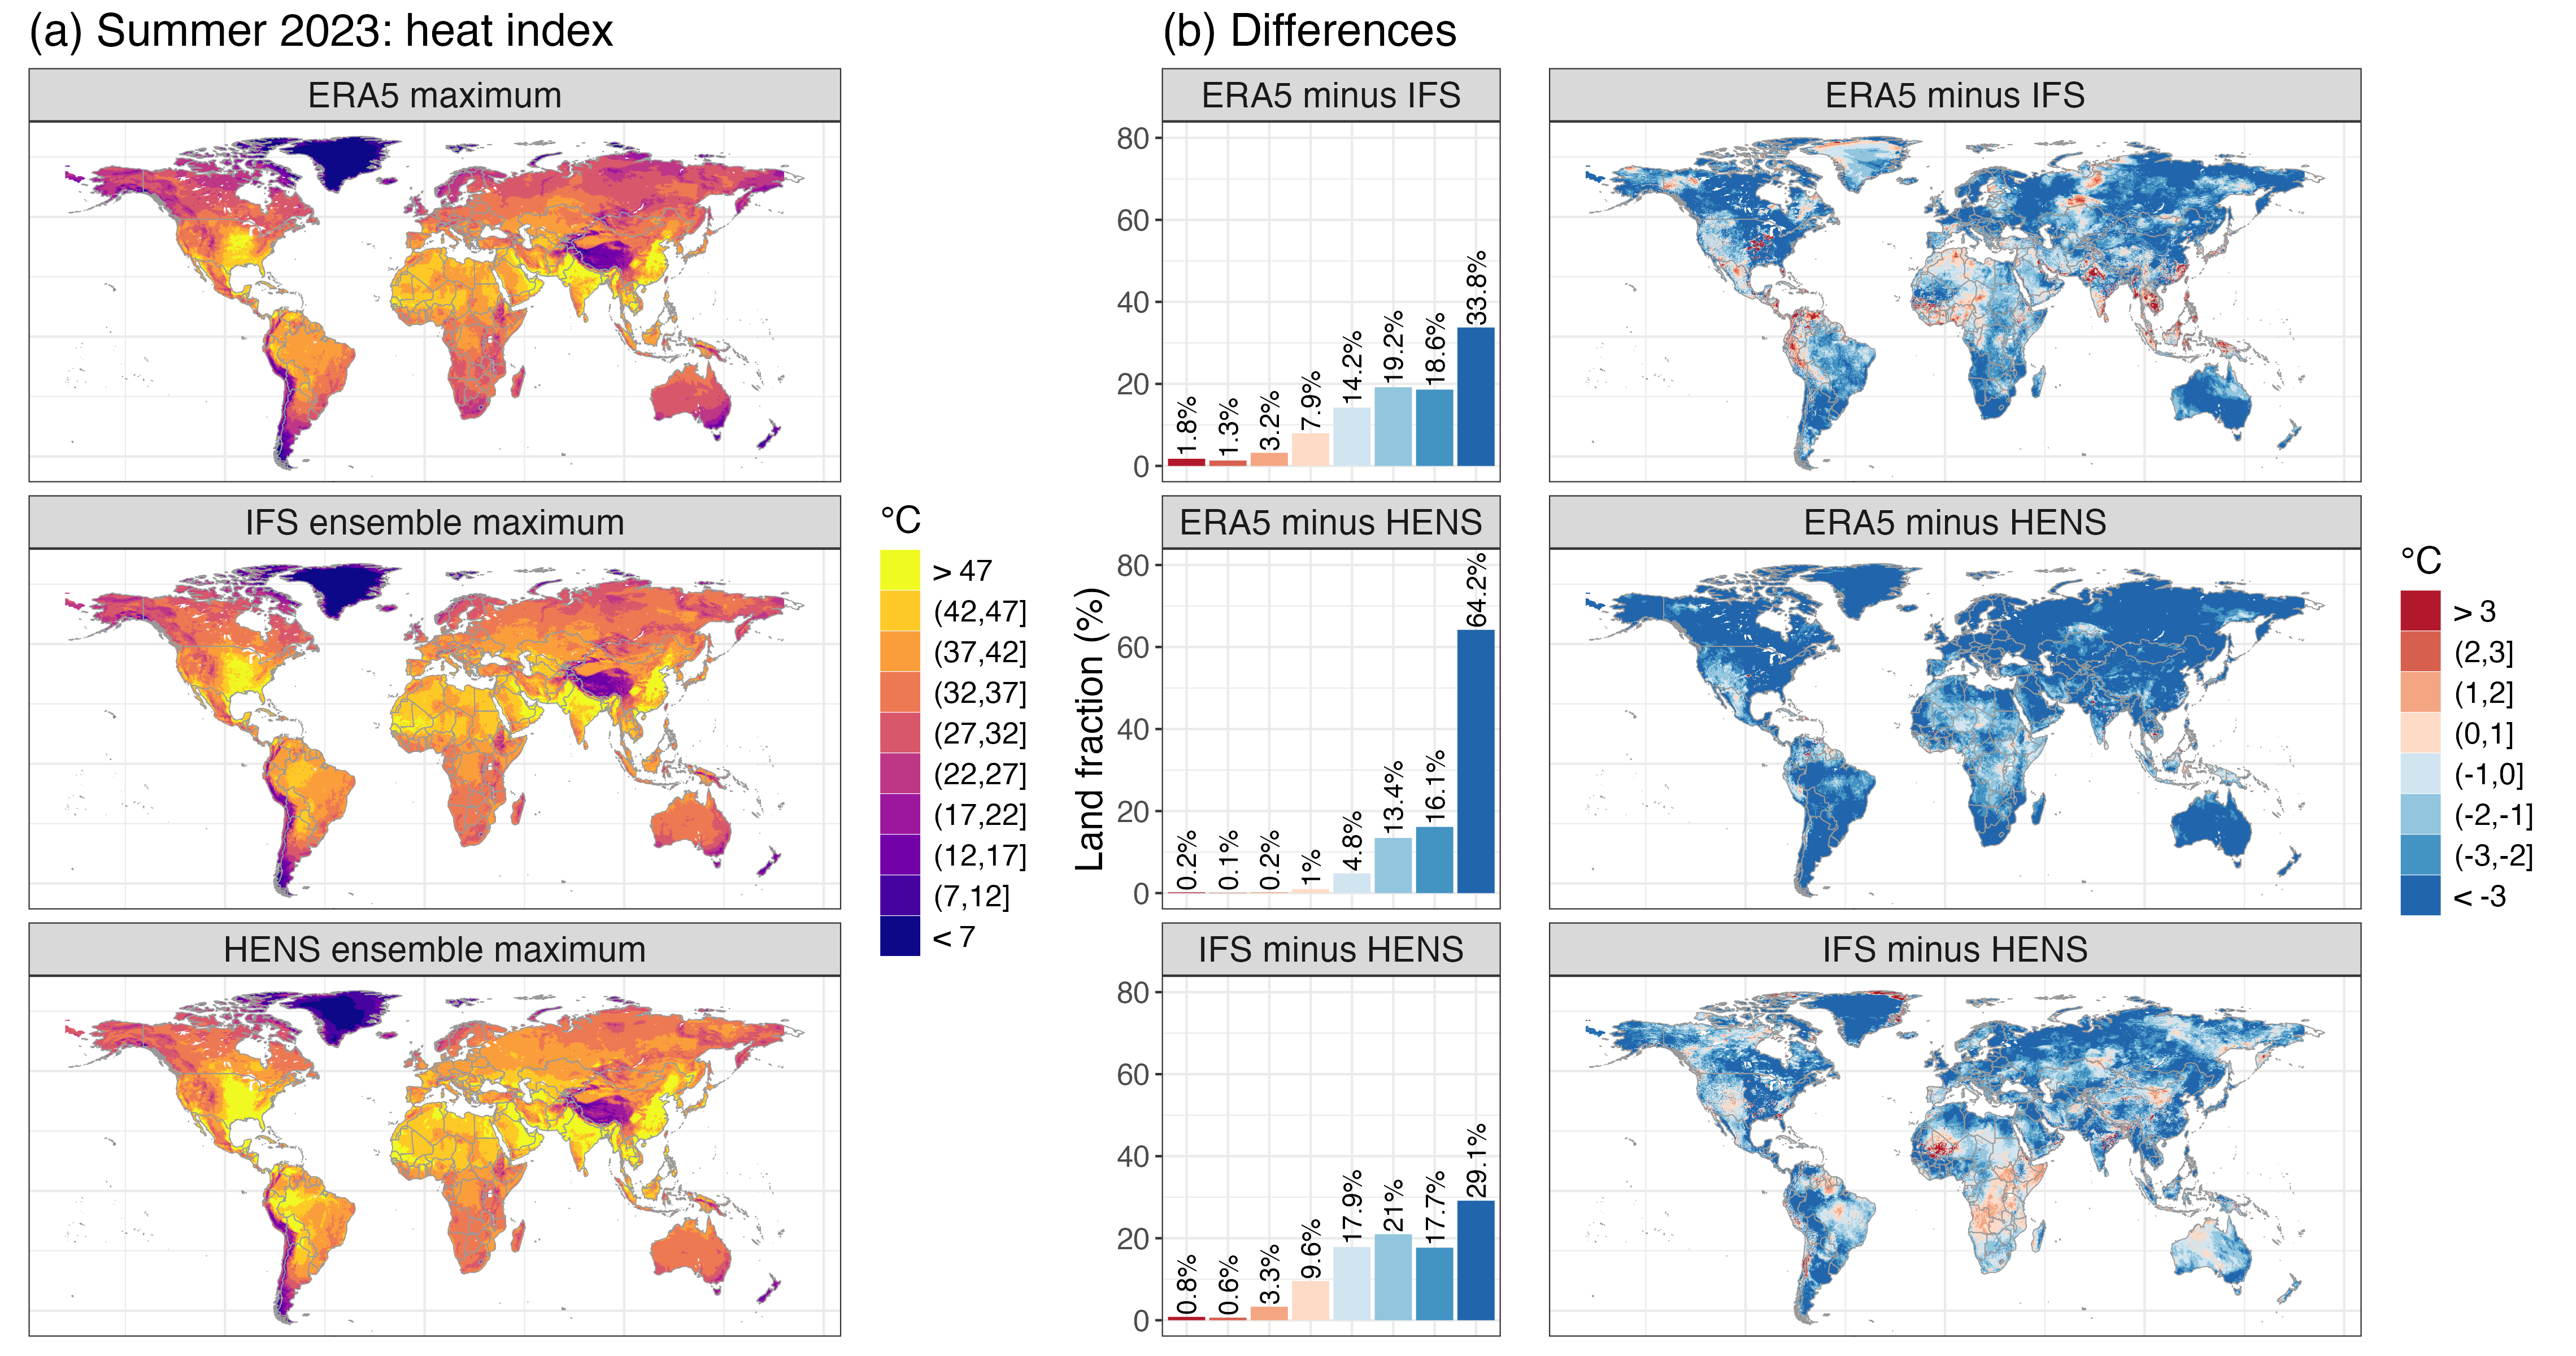
\includegraphics[width = \textwidth]{Figure_heatindex_maxima_diff.png}
\caption{Same as Figure 1 in the main text but for the heat index.}
\label{fig:threeversions_heatindex}
\end{figure*}

\begin{figure*}[!t]
\centering
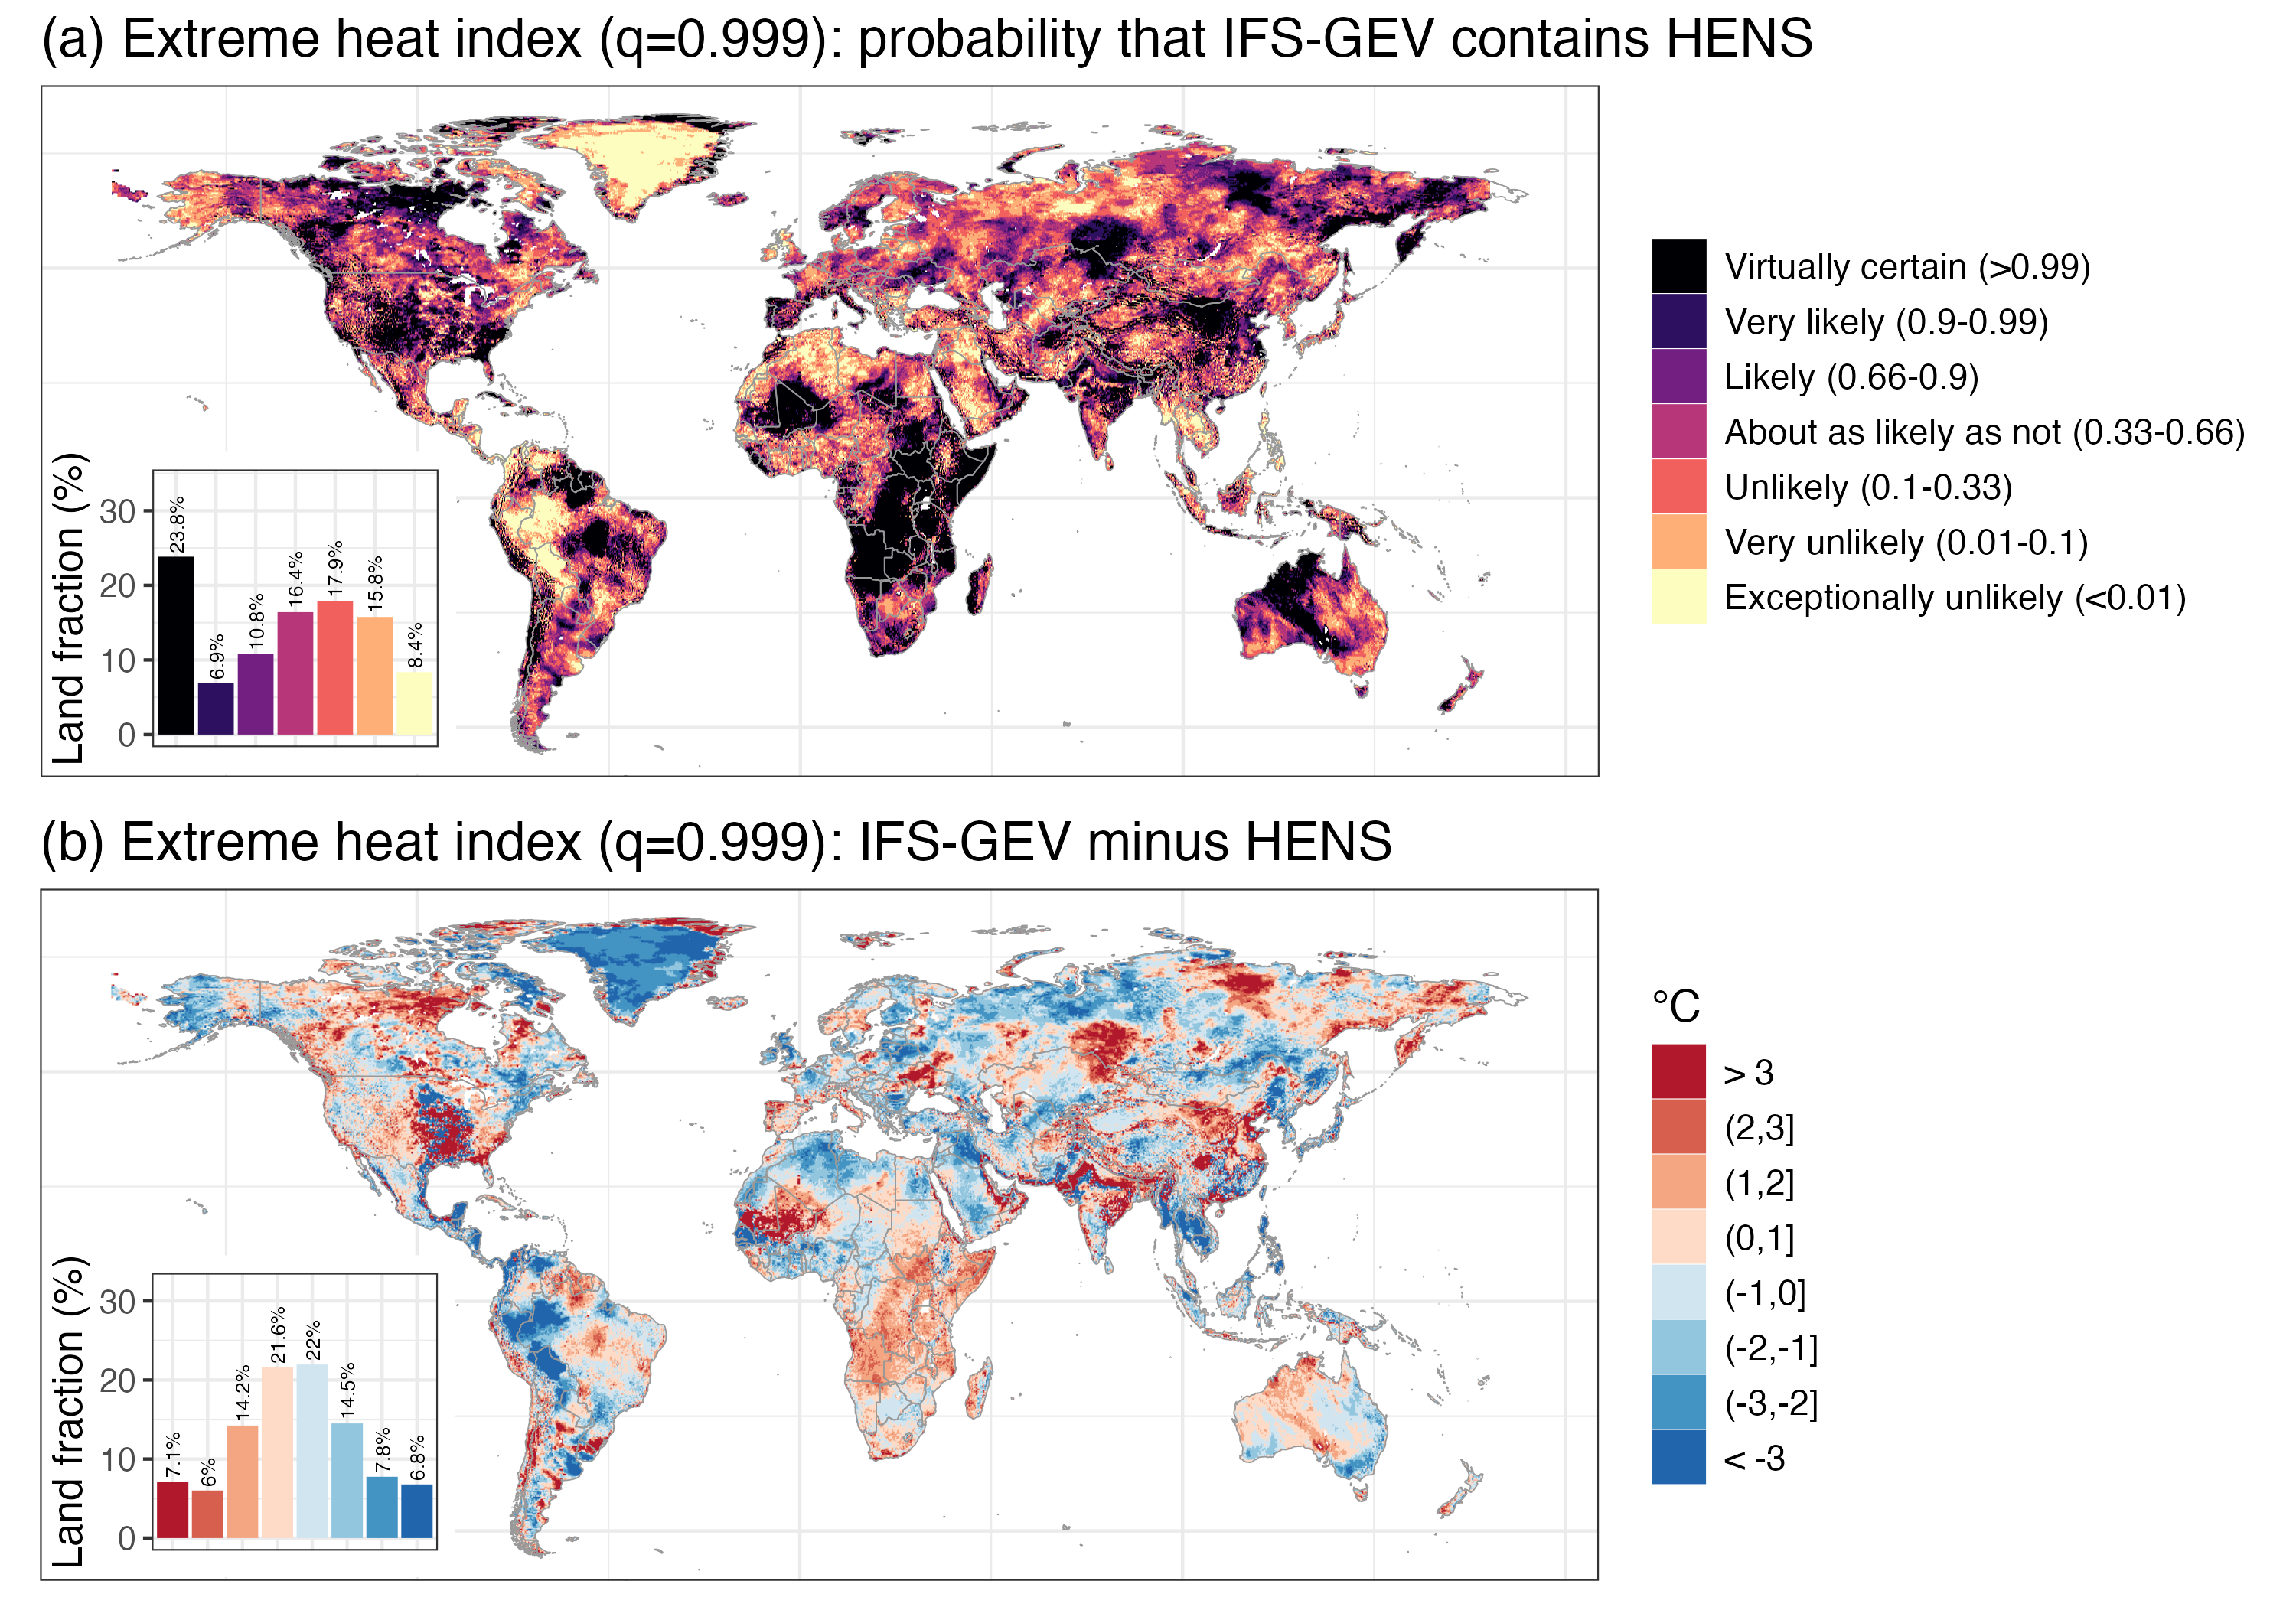
\includegraphics[width = \textwidth]{Figure_heatindex_probContain_1000day.png}
\caption{Comparison of IFS-GEV extreme event thresholds ($99.9\%$ percentile) for the heat index with corresponding empirical estimates calculated from the HENS ensemble. Panel (a) tallies the probability that the IFS-GEV threshold contains (is larger than) the HENS threshold; lighter colors indicate that HENS values are more extreme than IFS-GEV. Panel (b) tallies the difference in the IFS-GEV event threshold (the posterior median) and the HENS estimate. Panel insets show the land fraction in each color category.}
\label{fig:probcontain_hi}
\end{figure*}

% \begin{figure}
%     \centering
%     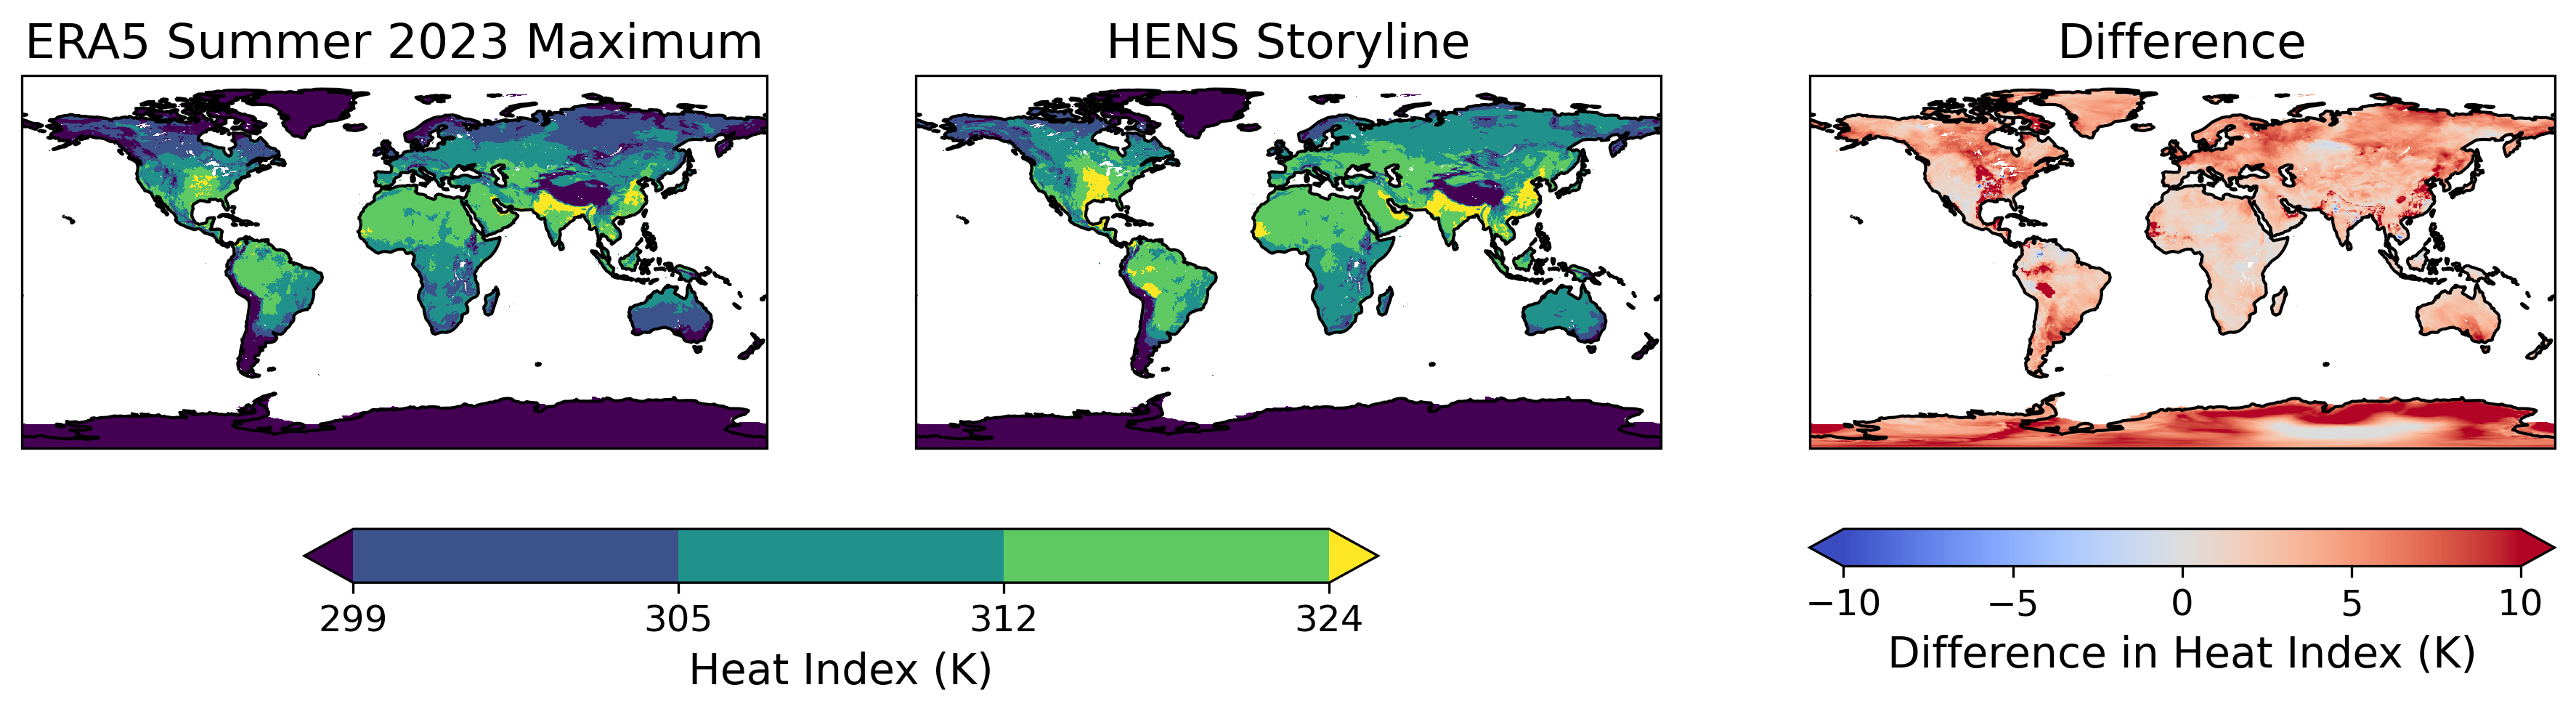
\includegraphics[width=\linewidth]{figures/era5_vs_hens_heatindex_with_diff.png}
%     \caption{ERA5 vs. HENS Storyline}
%     \label{fig:era5_vs_hens_heatindex_binned_nws}
% \end{figure}

% \begin{figure}
%     \centering
%     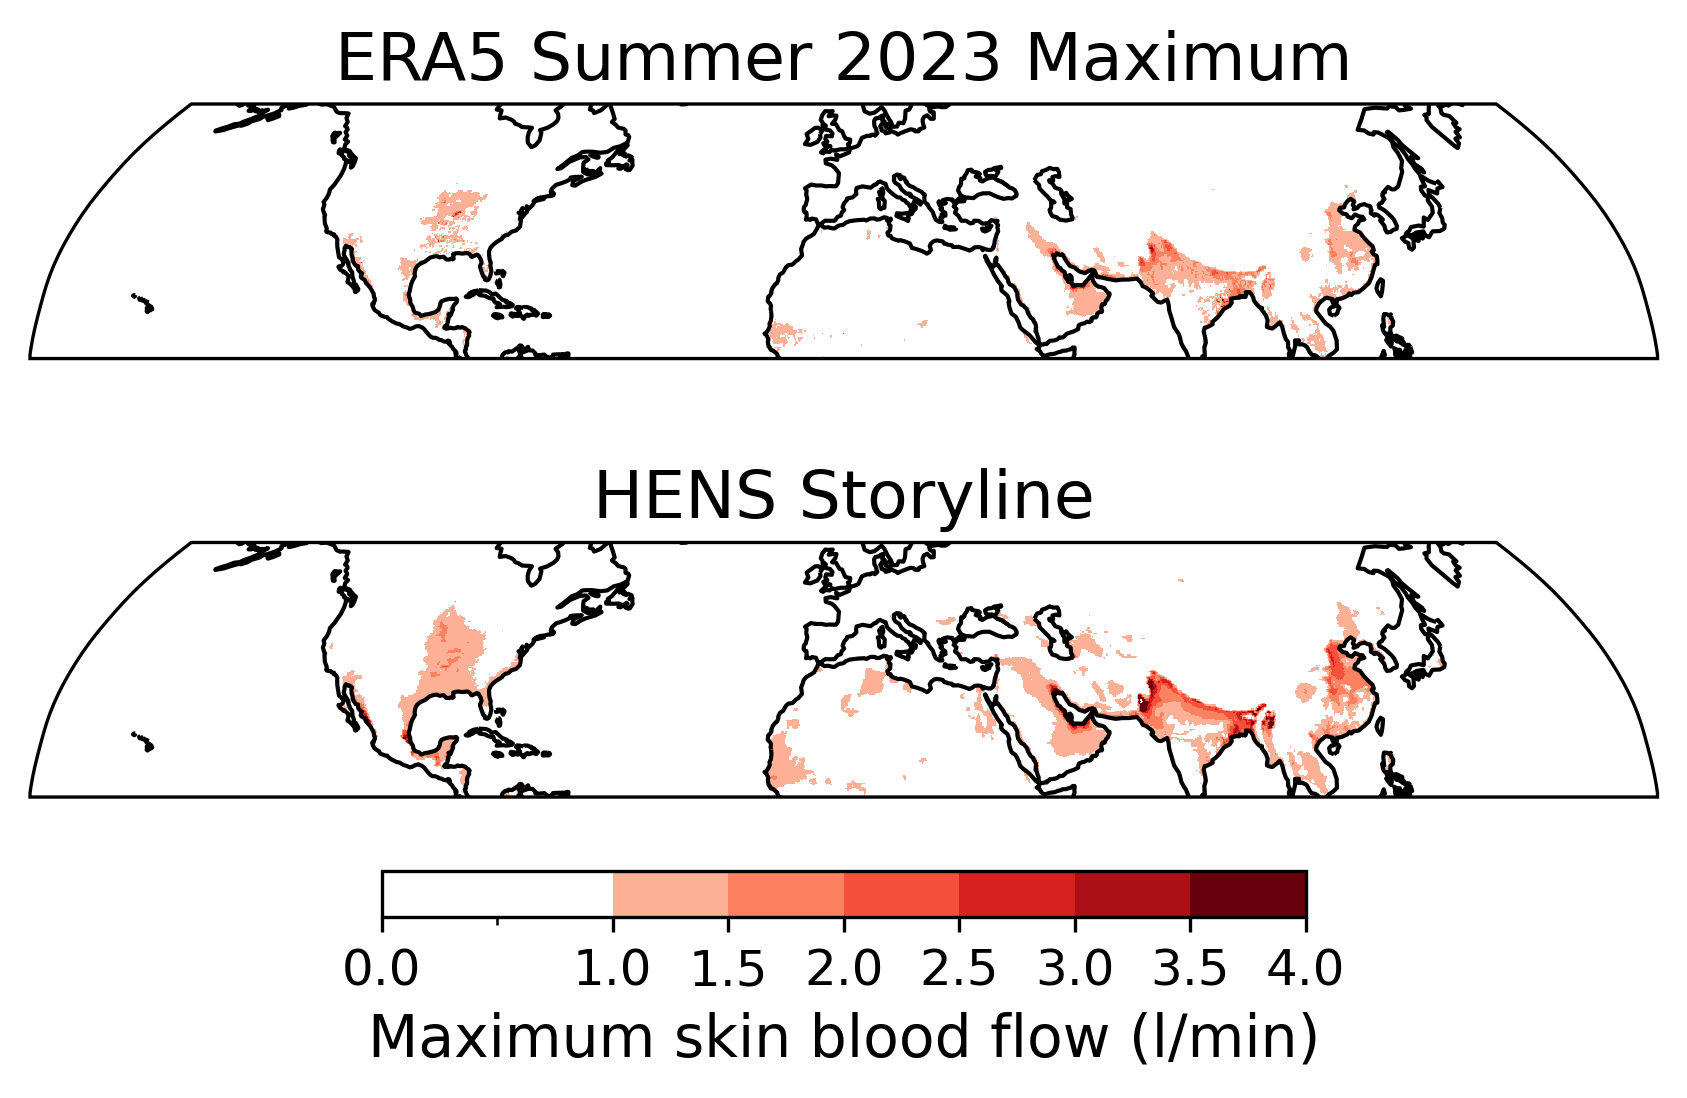
\includegraphics[width=\linewidth]{figures/blood_flow_figure.png}
%     \caption{ERA5 vs. HENS Storyline of maximum skin blood flow.}
%     \label{fig:era5_vs_hens_blood_flow}
% \end{figure}


% \begin{figure}[!h]
%     \centering
%     \includegraphics[width=\textwidth]{Figure_IFS_GEV_probContain_HENS.jpg}
%     \caption{As in Figure~\ref{fig:probcontain}(a) but for $r$-day return levels with $r\in\{100,1000,2000,\infty\}$.}
%     \label{supp:fig:probcontain}
% \end{figure}

% \begin{figure}[!h]
%     \centering
%     \includegraphics[width=\textwidth]{Figure_IFS_GEV_diff_HENS.jpg}
%     \caption{As in Figure~\ref{fig:probcontain}(b) but for $r$-day return levels with $r\in\{100,1000,2000,\infty\}$.}
%     \label{supp:fig:diff}
% \end{figure}

\clearpage

\section{Supplemental tables}

\begin{table}[!h]
\caption{Variables saved in the HENS Output.}
\centering
\begin{tabular}{l l l c}
\hline
\textbf{Variable}          & \textbf{Units}            & \textbf{Description}                    \\ \hline
\texttt{t2m}               & K                        & 2m temperature                          \\
\texttt{d2m}               & K                        & 2m dew point temperature                \\ 
\texttt{tcwv}              & kg/m²                    & Total column water vapor                \\
\texttt{t850}              & K                        & Temperature at 850 hPa                  \\
\texttt{z500}              & m²/s²                    & Geopotential at 500 hPa                 \\
\texttt{z300}              & m²/s²                    & Geopotential at 300 hPa                 \\
\texttt{msl}               & Pa                       & Mean sea level pressure                 \\
\texttt{t500}              & K                        & Temperature at 500 hPa                  \\
\texttt{sp}                & Pa                       & Surface pressure                        \\
\texttt{ivt}               & kg/(m·s)                 & Integrated vapor transport              \\
\texttt{heat\_index}       & K                        & Heat index                              \\
\texttt{wind\_speed10m}       & m/s                      & 10m wind speed                          \\ \hline
\end{tabular}
\label{table:variables}
\end{table}


\begin{table}[!h]
    \centering
    \begin{tabular}{c c}
 \hline
\textbf{HENS quantile} & \textbf{Fraction of ERA5 t2m maximum contained by HENS} \\ \hline
      $1 - 1/10 = 0.9$   &         $0.790$ \\
     $1 - 1/20 = 0.95$   &         $0.854$ \\
     $1 - 1/50 = 0.98$   &         $0.906$ \\
    $1 - 1/100 = 0.99$   &         $0.932$ \\
  $1 - 1/1000 = 0.999$   &         $0.978$ \\
 $1 - 1/2000 = 0.9995$   &         $0.984$ \\ 
 $1 - 1/5000 = 0.9998$   &         $0.989$ \\
Ensemble maximum & $0.994$ \\ \hline
    \end{tabular}
    \caption{The land fraction of the globe for which the 2m temperature HENS quantile contains the ERA5 summertime maximum t2m. We note that the containment fraction levels out for quantiles beyond $0.999$ (percentiles beyond $99.9\%$).}
    \label{tab:henscontain}
\end{table}

 %    Quantile FracContain_era5
 %      1 - 1/10 = 0.9            0.790
 %     1 - 1/20 = 0.95            0.854
 %     1 - 1/50 = 0.98            0.906
 %    1 - 1/100 = 0.99            0.932
 %  1 - 1/1000 = 0.999            0.978
 % 1 - 1/2000 = 0.9995            0.984
 % 1 - 1/5000 = 0.9998            0.989
 %       Ensemble max.            0.994

\clearpage
\bibliography{agusample}
\bibliographystyle{apalike}

\end{document}



More Information and Advice:

%% ------------------------------------------------------------------------ %%
%
%  SECTION HEADS
%
%% ------------------------------------------------------------------------ %%

% Capitalize the first letter of each word (except for
% prepositions, conjunctions, and articles that are
% three or fewer letters).

% AGU follows standard outline style; therefore, there cannot be a section 1 without
% a section 2, or a section 2.3.1 without a section 2.3.2.
% Please make sure your section numbers are balanced.
% ---------------
% Level 1 head
%
% Use the \section{} command to identify level 1 heads;
% type the appropriate head wording between the curly
% brackets, as shown below.
%
%An example:
%\section{Level 1 Head: Introduction}
%
% ---------------
% Level 2 head
%
% Use the \subsection{} command to identify level 2 heads.
%An example:
%\subsection{Level 2 Head}
%
% ---------------
% Level 3 head
%
% Use the \subsubsection{} command to identify level 3 heads
%An example:
%\subsubsection{Level 3 Head}
%
%---------------
% Level 4 head
%
% Use the \subsubsubsection{} command to identify level 3 heads
% An example:
%\subsubsubsection{Level 4 Head} An example.
%
%% ------------------------------------------------------------------------ %%
%
%  IN-TEXT LISTS
%
%% ------------------------------------------------------------------------ %%
%
% Do not use bulleted lists; enumerated lists are okay.
% \begin{enumerate}
% \item
% \item
% \item
% \end{enumerate}
%
%% ------------------------------------------------------------------------ %%
%
%  EQUATIONS
%
%% ------------------------------------------------------------------------ %%

% Single-line equations are centered.
% Equation arrays will appear left-aligned.

Math coded inside display math mode \[ ...\]
 will not be numbered, e.g.,:
 \[ x^2=y^2 + z^2\]

 Math coded inside \begin{equation} and \end{equation} will
 be automatically numbered, e.g.,:
 \begin{equation}
 x^2=y^2 + z^2
 \end{equation}


% To create multiline equations, use the
% \begin{eqnarray} and \end{eqnarray} environment
% as demonstrated below.
\begin{eqnarray}
  x_{1} & = & (x - x_{0}) \cos \Theta \nonumber \\
        && + (y - y_{0}) \sin \Theta  \nonumber \\
  y_{1} & = & -(x - x_{0}) \sin \Theta \nonumber \\
        && + (y - y_{0}) \cos \Theta.
\end{eqnarray}

%If you don't want an equation number, use the star form:
%\begin{eqnarray*}...\end{eqnarray*}

% Break each line at a sign of operation
% (+, -, etc.) if possible, with the sign of operation
% on the new line.

% Indent second and subsequent lines to align with
% the first character following the equal sign on the
% first line.

% Use an \hspace{} command to insert horizontal space
% into your equation if necessary. Place an appropriate
% unit of measure between the curly braces, e.g.
% \hspace{1in}; you may have to experiment to achieve
% the correct amount of space.


%% ------------------------------------------------------------------------ %%
%
%  EQUATION NUMBERING: COUNTER
%
%% ------------------------------------------------------------------------ %%

% You may change equation numbering by resetting
% the equation counter or by explicitly numbering
% an equation.

% To explicitly number an equation, type \eqnum{}
% (with the desired number between the brackets)
% after the \begin{equation} or \begin{eqnarray}
% command.  The \eqnum{} command will affect only
% the equation it appears with; LaTeX will number
% any equations appearing later in the manuscript
% according to the equation counter.
%

% If you have a multiline equation that needs only
% one equation number, use a \nonumber command in
% front of the double backslashes (\\) as shown in
% the multiline equation above.

% If you are using line numbers, remember to surround
% equations with \begin{linenomath*}...\end{linenomath*}

%  To add line numbers to lines in equations:
%  \begin{linenomath*}
%  \begin{equation}
%  \end{equation}
%  \end{linenomath*}



